\chapter{Шкоднае асяродзьдзе}

\section{Нашае асяродзьдзе і здароўе}

Кожны месяц мы робім мільён удыхаў і выдыхаў, і якасьць паветра вакол нас уплывае на наша здароўе, стан розуму і цела. Стан паветра ў~памяшканьні можа быць у~2--5 разоў горшы, чым звонку, прычым гэта ня толькі сучасная праблема: у~старажытнасьці людзі пакутавалі ад лішку дыму, абаграваючы свае хаты агмянямі без камінаў і паўнавартасных печаў. Актуальны чыньнік~--- гэта шум, якога становіцца ўсё больш у~нашых гарадах і які не змаўкае нават ноччу, а~таксама лішак сьвятла і цяпла. Уплывае на наша здароўе і электрамагнітнае выпраменьваньне. Навакольнае асяродзьдзе інтэнсіўна забруджваецца таксінамі: плястык, цяжкія мэталы, бісфэнолы, антыбіётыкі і інш. Для падтрыманьня і ўмацаваньня здароўя нам важна ня толькі займацца сабой, але й мяняць навакольнае асяродзьдзе, зь якім мы так шчыльна злучаныя. Калі гены памяняць нельга, звычкі~--- цяжка, то асяродзьдзе~--- куды лягчэй.

\textbf{Ня толькі мы ўплываем на асяродзьдзе~--- асяродзьдзе ўплывае на нас.} Уявіце сабе чалавека, які жыве ва ўласнай хаце ці малапавярховай забудове, далёка ад магістралі, з~зручнымі для шпацыраў ці прабежак сьцежкамі, дзе шмат дрэваў, чыстае паветра, ціхія вуліцы і знаёмыя суседзі. У такім асяродзьдзі ўсё цешыць вашае вока, разьнявольвае, тут хочацца выходзіць на вуліцу і шпацыраваць, спыняцца для сяброўскіх гутарак, любавацца прыродай, займацца спортам на турніках~--- усё гэта аўтаматычна спрыяе здароўю.

Калі ж чалавек жыве ва ўмовах цясноцьця сучаснага індустрыяльнага горада, то навакольнае асяродзьдзе, хутчэй за ўсё, узмацняе стрэс і шкодзіць здароўю: шматпавярховая забудова, вузкія тратуары, сьмецьце на вуліцах, надпісы на сьценах, шмат незнаёмцаў (і маргіналы сустракаюцца), шчыльны рух аўтамабіляў, адсутнасьць паркаў і пешаходнай інфраструктуры, пастаянны шум, бруднае паветра, мала зеляніны, позірк упіраецца ў~бэтонныя агароджы і парэпаную тынкоўку. У такім асяродзьдзі не ўзьнікае ані найменшага жаданьня выходзіць на вуліцу, і чалавек праводзіць вольныя гадзіны на канапе побач з~кампутарам і лядоўняй, бо гэта куды больш бясьпечны і прыемны спосаб баўленьня часу ў~такой сытуацыі.

\begin{figure}[htb!]
  \centering
  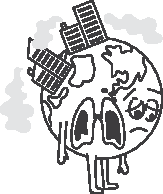
\includegraphics[scale=1.5]{willpower/ch11/1.pdf}
\end{figure}

\emph{У розныя часы асяродзьдзе ўяўляла розныя пагрозы. У самым пачатку сваёй эвалюцыі чалавек пачаў актыўнае пераўтварэньне навакольнага асяродзьдзя ў~сваіх інтарэсах, выкарыстоўваючы агонь, інструмэнты, аб'ядноўваючы намаганьні супляменьнікаў. Цясноцьце ў~старажытных гарадах і антысанітарыя спрыялі разьвіцьцю эпідэміяў і паразітарных інфэкцыяш, і неабходнасьць супрацьстаяць хваробам і выжываць прысьцёбвала далейшае разьвіцьцё.}

У апошнюю сотню гадоў людзі неймаверна хутка мяняюць навакольнае асяродзьдзе, мы не пасьпяваем адаптавацца, і гэтыя зьмены ня йдуць на карысьць нашаму здароўю. Мы пазбаўляемся шэрагу карысных чыньнікаў навакольнага асяродзьдзя, такіх як сонца, моцна ўзьдзейнічаюць шкодныя фактары, напрыклад бруднае паветра. Для многіх таксінаў і сьмецьця не існуе дзяржаўных межаў~--- яны разьмяркоўваюцца па ўсёй плянэце, назапашваюцца ў~глебе, расьлінах і жывёлах і трапляюць у~наш арганізм. Паветраныя таксіны таксама разносяцца па ўсёй зямной кулі і ўзьдзейнічаюць на ўсіх людзей.

На працягу свайго жыцьця мы жывём у~розных месцах і часта выбіраем іх выпадкова. Нават у~рамках аднаго дня мы бываем у~пэўнай колькасьці месцаў. Прааналізуйце іх і падумайце, як яны ўплываюць на ваша здароўе. Магчыма, частку гэтых месцаў можна зьмяніць на больш здаровыя?

\textbf{Аптымальныя ўмовы навакольнага асяродзьдзя}~--- гэта такое асяродзьдзе, у~якім у~нас выяўляецца аптымальнае самаадчуваньне, мінімальная рызыка захворваньняў і высокая працягласьць жыцьця. Вельмі часта сацыяльныя (атачэньне), фізычныя (шум, сьвятло, тэмпэратура, выпраменьваньне), хімічныя (паветра, вада, прадукты) і біялягічныя (цьвіль, паразіты) чыньнікі злучаюцца і дзейнічаюць разам. Таму важна падтрымліваць гігіену навакольнага асяродзьдзя. Вялікае значэньне мае мікраклімат у~кватэры і хаце. Спалучэньне неспрыяльных аздобных матэрыялаў, тэмпэратуры, вільготнасьці, вэнтыляцыі можа прывесьці да сындрому ``хворага дому'', які разбурае здароўе сваіх насельнікаў і кароціць жыцьцё.

Многія людзі зьвяртаюцца да розных спосабаў ``дэтаксікацыі'', але, па сутнасьці, самы надзейны спосаб паменшыць таксічную нагрузку~--- гэта зьнізіць трапленьне шкодных рэчываў у~арганізм, то бок палепшыць асяродзьдзе, у~якім мы жывём. Наша мэта~--- навучыцца ў~любым месцы выяўляць шкодныя чыньнікі асяродзьдзя і ліквідаваць іх, плюс папоўніваць брак карысных чыньнікаў у~сваім асяродзьдзі для фармаваньня аптымальных умоваў.

\begin{figure}[htb!]
  \centering
  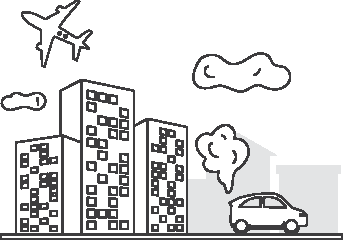
\includegraphics[scale=1.3]{willpower/ch11/2.pdf}
\end{figure}

\subsection*{Пытаньні і заданьні}

1. Ацаніце бясьпеку навакольнага асяродзьдзя ў~месцы, дзе вы жывяце.

2. Што з~чыньнікаў асяродзьдзя вакол вас падаецца самым небясьпечным? Як гэта можна зьмяніць?

3. У якім месцы і асяродзьдзі вы б хацелі жыць? Апішыце ваш ідэальны дом, мястэчка, горад, краіну.


\section{Бруднае паветра і здароўе}

Многія людзі лічаць, што ім бракуе кіслароду ў~памяшканьні або на вуліцы, хоць рэальная прычына нядужаньня, як правіла, зусім іншая~--- забруджваньне паветра або сындром гіпэрвэнтыляцыі (пачашчанае дыханьне пры стрэсе, якое можа прывесьці да галавакружэньня).

\infobox{Бруднае паветра~--- адзін з~самых небясьпечных шкоднасных чыньнікаў навакольнага асяродзьдзя.}

\emph{Сур'ёзнае навуковае вывучэньне шкоды бруднага паветра пачалося ў~1952 годзе, калі Лёндан накрыў смог ад спальваньня вугалю, што прывяло да тысячаў сьмерцяў. З таго часу чысьціня паветра стала рэгулявацца заканадаўча, але да вырашэньня праблемы нам далёка.}

Нягледзячы на забарону спальваньня вугалю, праблема бруднага паветра становіцца ўсё больш актуальнай праз павелічэньне колькасьці транспарту і працы заводаў. Больш за 90\,\% жыхароў плянэты сутыкаюцца з~праблемай забруджваньня паветра. Апроч вонкавага забруджваньня існуе і ўнутранае, калі ў~жылых памяшканьнях паляць, гатуюць ежу, топяць печы з~дрэннай вэнтыляцыяй, паляць духмянкі і г.~д.

\subsection*{У 30 разоў танчэй за волас!}

Мацней за ўсё на нас уплываюць дробныя часьціцы, якія ўтвараюцца пры згараньні паліва. Яны разносяцца са струмянямі паветра, доўгі час не асядаючы на зямлю. Узважаныя часьціцы ўяўляюць сабой складаную сумесь, якая можа патрапіць глыбока ў~лёгкія, а~празь іх~--- у~кроў.

\emph{Вылучаюць дзьве яе асноўныя разнавіднасьці: PM10 часьціцы, дыямэтрам менш за 10\,мкм, і PM2,5 часьціцы, дыямэтрам менш за 2,5\,мкм. Уявіце сабе волас, дык вось часьціца PM10 у~сем разоў меншая за яго дыямэтар, а~PM 2,5~--- меншая ў~30 разоў. Чыстым лічыцца паветра са сярэднегадавым утрыманьнем часьціц PM 2,5 у~паветры 10\,мкг/м\textsuperscript{3} і сярэднясутачным 25\,мкг/м\textsuperscript{3}.}

Часьціцы валодаюць рознымі па складзе кампанэнтамі: яны могуць утрымоўваць мэталы (Fe, Ni, Cu, Co, Cr), араматычныя гідракарбоны, эндатаксіны і да т.~п. Таксама ў~паветры можа быць шмат іншых забруджвальнікаў: бэнзапірэн, які ўтвараецца пры згараньні цьвёрдага паліва, сажысты вуглярод, прыземны азон, аксіды азоту, двухвокіс серы і інш. Як жартуюць жыхары мэгаполісаў, «ня толькі дыхаеш сьвежым паветрам на вуліцы, але і насычаесься мікраэлемэнтамі».

\textbf{Чым небясьпечна?} Бруднае паветра зьвязанае з~16\,\% усіх сьмерцяў, што практычна ў~15 разоў больш, чым гіне сёньня ва ўсім сьвеце ад войнаў і іншых формаў гвалту. Бруднае паветра скарачае працягласьць жыцьця больш чым на год. Высокі ўзровень часьціц PM2.5 адказны за 3\,\% усіх сардэчна-сасудзістых сьмерцяў і за 5\,\% сьмерцяў ад раку лёгкіх.

\infobox{У самых забруджаных гарадах вырашэньне праблемы магло б павялічыць чаканую працягласьць жыцьця на 20 месяцаў.}

Бруднае паветра выклікае хуткія і павольныя зваротныя рэакцыі. Хуткая рэакцыя зьвязаная з~раздражненьнем рэцэптараў лёгкіх, а~павольны адказ~--- з~павелічэньнем ўзроўню хранічнага запаленьня і ўзроўню С-рэактыўнага бялку. Кожныя дадатковыя 5\,мкг/м\textsuperscript{3} часьціц на 1,3\,\% павялічваюць узровень С-рэактыўнага бялку. А запаленьне, як мы ведаем, павялічвае рызыку шматлікіх захворваньняў і паскарае старэньне, узмацняючы згусальнасьць крыві, павялічваючы канцэнтрацыю фібрынагену. Бруднае паветра зьвязанае з~павелічэньнем таўшчыні комплексу інтым-мэдыя (маркер прагрэсаваньня атэрасклерозу) і павялічвае рызыку інсульту і інфаркту. Таксама забруджваньне паветра павялічвае рызыку дыябэту, прыводзіць да зьніжэньня адчувальнасьці да інсуліну, пагаршае якасьць сну, зьніжае функцыі нырак.

Небясьпечным зьяўляецца і кароткачасовае забруджваньне: пры рэзкім забруджваньні паветра павялічваецца колькасьць шпіталізацый з~астмай, пнэўманіяй, абструктыўнай хваробай лёгкіх, сардэчнымі прыступамі. Чым бруднейшае паветра ў~горадзе, тым больш небясьпечна ў~ім жыць.

\textbf{Уплыў на мозг.} Бруднае паветра пагаршае кагнітыўныя здольнасьці і памяншае ўзровень шчасьця, уплывае на мозг, зьмяншае прадукцыйнасьць, мяняе наша стаўленьне да рызыкі, павялічвае агрэсію і, як вынік, злачыннасьць. Запаленьне ад бруднага паветра зьвязана з~рызыкай дэпрэсіі і суіцыду: павелічэньне забруджваньня паветра на 10\,мкг/м\textsuperscript{3} на працягу трох дзён павышала рызыку самагубства на 2\,\%. Пражываньне паблізу ажыўленых трасаў павялічвае рызыку нэўрадэгенэратыўных захворваньняў.

\infobox{Рызыка хваробы Альцгаймэра на 12\,\% вышэйшая ў~тых, хто жыве за 50 мэтраў ад дарогі, у~параўнаньні з~тымі, хто жыве на адлегласьці 200 і больш мэтраў. Пятая частка ўсіх выпадкаў захворваньняў можа быць выклікана брудным паветрам.}

\begin{figure}[htb!]
  \centering
  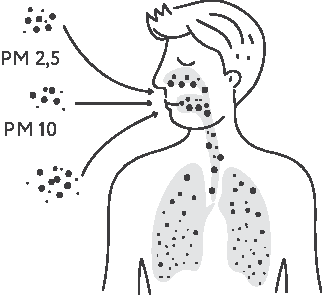
\includegraphics[scale=1.3]{willpower/ch11/3.pdf}
\end{figure}

Асабліва адчувальныя да бруднага паветра дзеці, цяжарныя, старыя, людзі з~хранічнымі захворваньнямі. Часьціцы сажы могуць патрапіць нават у~пляцэнту~--- так, забруджваньне павялічвае рызыку заганаў разьвіцьця, выклікае затрымку росту і зьніжэньне аб'ёму мозгу ў~дзяцей, пагаршэньне іх псыхічнага здароўя, уключаючы рызыку дзіцячых дэпрэсій. У розных дасьледаваньнях бруднае паветра павялічвае рызыку аўтызму ад 12 да 76\,\%. Дасьледаваньні на жывёлах пацьвярджаюць, што пражываньне паблізу ажыўленых трасаў шкодзіць мозгу нашчадкаш яшчэ на раньніх стадыях разьвіцьця, павялічваючы ўзровень нэўразапаленьня.

\subsection*{Пытаньні і заданьні}

1. Як мяняецца ваша самаадчуваньне пры доўгім знаходжаньні ва ўмовах забруджанага паветра?

2. Ці заўважаеце вы розьніцу якасьці паветра ў~горадзе і за яго межамі?

3. Ці шмат часу вы праводзіце ў~транспарце?


\section{Барацьба з~брудным паветрам}

\emph{Джэнтльмэн у~5 гадзінаў раніцы вывальваецца з~бару і зьдзіўлена пытаецца: ``Швайцар, што за дзіўны пах?''~--- ``Гэта чыстае паветра, сэр''.}

Спадзявацца на свае органы пачуцьцяў для ацэнкі паветра не заўсёды добрая ідэя, бо мы прыстасоўваемся да любога асяродзьдзя і перастаём заўважаць працягла дзейсныя раздражняльнікі. Таму нам патрэбныя аб'ектыўныя спосабы вымярэньня якасьці паветра.

Першае, з~чаго трэба пачаць, гэта весьці маніторынг якасьці паветра. У гарадах, дзе шмат датчыкаў, можна скарыстацца мапамі, на якіх выводзяцца штохвілінныя паказьнікі, і ўсталяваць іх на тэлефон. Калі ў~вашым горадзе такой сыстэмы датчыкаў няма ці вы хочаце атрымаць высокую дакладнасьць вымярэньняў, то можна набыць датчык якасьці паветра для сябе~--- абавязкова з~вымярэньнем колькасьці часьціц P2,5. Многія датчыкі сынхранізуюцца са смартфонамі, і канкрэтныя лічбы будуць заўсёды ў~вас пад рукой. Некаторыя вытворцы дазваляюць уключыць свой датчык у~глябальную сетку, напрыклад, AirVision. Так ваша вымярэньне становіцца даступным і для людзей побач.

\textbf{Скарачайце ўзьдзеяньне.} Уплыў забруджанага паветра мае назапашвальны эфэкт~--- гэта значыць, чым больш узровень і даўжэй узьдзеяньне, тым горш. Калі мінімізаваць узьдзеяньне бруднага паветра і дыхаць чыстым паветрам дома, то арганізм пасьпявае выводзіць тое, што патрапіла на вуліцы. Трымайцеся далей ад дарог, асабліва буйных.

\begin{figure}[htb!]
  \centering
  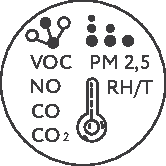
\includegraphics[scale=1.5]{willpower/ch11/4.pdf}
\end{figure}

\textbf{Кожны мэтар мае значэньне}, бо з~аддаленьнем ад крыніцы забруджваньне скарачаецца экспанентна, выхлапы разводзяцца чыстым паветрам. Гуляйце ці рабіце прагулкі не ў~гадзіну пік і не адразу ж пасьля яе заканчэньня. Калі вы ідзяце з~маленькімі дзецьмі, то паднімайце іх на рукі, каб трымаць вышэй за ўзровень выхлапных газаў. Ня стойце каля самай дарогі, калі чакаеце зялёнага сыгнала сьвятлафора. Памятайце, што важная ня проста адсутнасьць трасы або завода побач, але і кірунак ветру. Калі праз надвор'е, слабы вецер ці пажары ў~горадзе паўстаў смог, па магчымасьці выязджайце за горад ці трымайце дома ўключаны фільтр ачысткі паветра (пра фільтры ніжэй) пры закрытых вокнах.

Аптымізуйце маршруты для прагулак і прабежак, выбірайце аддаленыя зялёныя вулачкі, гэта можа зьнізіць узьдзеяньне бруднага паветра на 50--60\,\%.

\infobox{Будзе выдатна, калі навігатары навучацца пракладаць ня толькі самы хуткі, але й самы ``зялёны'' маршрут.}

Гэтае правіла тычыцца і кіроўцаў, бо доўгая дарога за рулём і заторы павялічваюць рызыку ўдыханьня бруднага паветра. Не прыціскайце нос свайго аўтамабіля да выхлапной трубы машыны, якая стаіць наперадзе. У заторы лепш закрыць вокны і адключыць вэнтыляцыю салёна, гэта дазволіць зьменшыць забруджваньне ад суседніх машын. Па магчымасьці, менш карыстайцеся аўтамабілем у~гадзіну пік. У некаторых машынах, напрыклад у~Tesla, усталяваныя вельмі якасныя фільтры салёна, зьвяртайце на гэта ўвагу пры выбары і абслугоўваньні аўто.

\textbf{Маскі.} Звычайныя маскі, якія няшчыльна прылягаюць да твару, маюць вельмі слабую эфэктыўнасьць, затрымліваючы толькі 20\,\% дробных часьціц. Выбірайце спэцыяльныя маскі з~маркіроўкай N95 або N99 (затрымліваюць 95 і 99\,\% часьціц 2.5). Улічвайце памер, зручнасьць, шчыльнасьць прыляганьня, працягласьць выкарыстаньня маскі, эфэктыўнасьць і тэрмін службы фільтраў. Звычайна такія маскі маюць працягласьць выкарыстаньня ня больш за 40 гадзінаў. Маркіроўка C абазначае вугальны фільтр, які затрымлівае азон або аксід серы, маркіроўка V~--- наяўнасьць клапана для вывядзеньня лішку вільготнасьці, Р~--- здольнасьць фільтраваць і арганічныя забруджвальнікі.

\textbf{Зніжэньне ўзьдзеяньня забруджанага паветра працуе.} Так, зьніжэньне канцэнтрацыі PM2,5 за ўсё на 2,5\,мкг/м\textsuperscript{3} прыводзіла да зьніжэньня сьмяротнасьці ад усіх прычынаў на 3,5\,\%. Шматразова апісаны выпадкі, калі спыненьне работы заводаў праз забастоўкі прыводзіла да зьніжэньня захваральнасьці ў~навакольных населеных пунктах у~некалькі разоў: зьніжалася частата астмы, бранхіту, кашлю, кан'юктывіту.

Уступайце ў~шэрагі грамадзянскіх актывістаў, патрабуйце ад мясцовых уладаў пераносу шкоднай прамысловасьці або ўстаноўкі ачышчальных збудаваньняў, стварэньня пешаходных вуліц, абмежаваньні руху асабістых аўтамабіляў, разьвіцьця грамадскага транспарту, пераходу на электрамабілі, барацьбы са спальваньнем паліва, ляснымі пажарамі.

\emph{Вядзеньне здаровага ладу жыцьця, у~прыватнасьці здаровае харчаваньне, дапамагае зьмякчыць узьдзеяньне бруднага паветра, бо шэраг прадуктаў валодае супрацьзапаленчымі ўласьцівасьцямі.}

Часам людзі лічаць, што яны могуць «прывыкнуць» да бруднага паветра, як у~анекдоце: «Ды як вы можаце дыхаць такім паветрам?~--- А мы не зацягваемся!». Але гэта небясьпечная памылка. Нават калі вы ня бачыце забруджваньня, гэта ня значыць, што яно ня шкодзіць вам.

\subsection*{У жылым памяшканьні}

Дома мы праводзім шмат часу, таму важна забясьпечыць там аптымальную якасьць паветра~--- і гэта вам па сілах. Бо лёгкія могуць пасьпяваць чысьціцца, пакуль вы сьпіце і адпачываеце ад гарадзкога паветра. Прытокавая вэнтыляцыя з~функцыяй ачысткі дапамагае забясьпечыць паўнавартасную ачыстку і зьмену паветра. Калі вы выкарыстоўваеце кандыцыянэр, то яго трэба рэгулярна чысьціць і мяняць фільтры, інакш на іх могуць запасіцца бактэрыі і цьвіль, якія затым разносяцца па пакоі. Рэгулярна запускайце рэжым вэнтыляцыі, каб не размнажалася цьвіль.

\infobox{Заўсёды гатуйце ежу пры ўключанай выцяжцы, пазьбягайце залішне паліць сьвечкі ці араматычныя палачкі, не карыстайцеся аэразолямі і араматызатарамі.}

Сачыце за тэхнічным станам награвальнікаў вады на газе, газавымі плітамі, абагравальнікамі і ўсімі прыборамі, дзе спальваецца паліва. Абмяжоўвайце колькасьць сынтэтычных мыйных сродкаў, лепш выкарыстоўваць ачыстку парай. Часьцей выносьце сьмецьце, трымайце бытавую хімію ў~старанна закаркаваных ёмістасьцях далей ад дзяцей.

\begin{figure}[htb!]
  \centering
  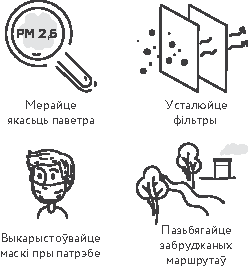
\includegraphics[scale=1.5]{willpower/ch11/5.pdf}
\end{figure}

\textbf{Усталюйце HEPA фільтр.} Гэтае простае і эфэктыўнае рашэньне, бо менавіта НЕРА фільтр лепш за ўсё чысьціць паветра ад небясьпечных РМ 2.5 часьціц і зьмяншае іх канцэнтрацыю. Пры гэтым кантралюйце эфэктыўнасьць ачысткі датчыкам РМ 2.5 (ён можа быць і ўбудаваны ў~фільтр). Дасьледаваньні паказваюць, што выкарыстаньне такіх фільтраў паляпшае якасьць сну. Асабліва яны важныя для дзяцей і цяжарных. Чыстае паветра ўначы вельмі важнае, бо гэта дае магчымасьць дыхальным шляхам ачысьціцца і хоць часткова кампэнсаваць дыханьне брудным паветрам днём.

Зьвярніце ўвагу, што з~цягам часу эфэктыўнасьць фільтраў зьмяншаецца, і іх важна мяняць. Калі вы жывяце ў~прыватным доме, то вялікая колькасьць дрэваў і кустоўя могуць захопліваць часьціцы і зьніжаць іх канцэнтрацыю ў~паветры.

\subsection*{Пытаньні і заданьні}

1. Ацаніце якасьць паветра дома і на вуліцы, выкарыстоўваючы грамадскія сыстэмы назіраньня або ўсталяваўшы ўласныя датчыкі. Таксама вы можаце далучыць праз інтэрнэт свой датчык да глябальнага анляйн-маніторынгу якасьці паветра, каб зрабіць гэтую інфармацыю даступнай для ўсіх.

2. Вывучыце карту вашага раёна: ці ёсьць побач прадпрыемствы? Вывучыце аб'ём выкідаў і ружу вятроў.

3. Пры неабходнасьці купіце ачышчальнік паветра для вашай кватэры. Адзначце, як зьмянілася ваша самаадчуваньне пры паляпшэньні якасьці паветра.


\section{Вуглякіслы газ у~памяшканьні}

У офісах увесь час ідуць бітвы паміж тымі, каму душна, і тымі, хто баіцца скавышоў. Ёсьць людзі, якія асабліва гостра адчуваюць якасьць паветра, а~ёсьць тыя, хто баіцца сьвежага паветра. Мы ўжо пагаварылі пра важнасьць чыстага паветра на вуліцы, але вялікае значэньне мае паветра, якім вы дыхаеце дома і на працы. Паветра ў~памяшканьні часта ў~некалькі разоў бруднейшае, чым звонку. Калі мы заходзім з~вуліцы ў~памяшканьне, то можам адчуць сьпёртасьць паветра, але гэтае адчуваньне хутка зьнікае~--- мы да яго звыкаем. 

\infobox{Сьпёртасьць~--- гэта часта лішак вуглякіслага газу, які выдыхаюць людзі. Гэта нябачны, але шкодны ў~высокіх канцэнтрацыях чыньнік.}

Сярэдняя канцэнтрацыя вуглякіслага газу (CO\textsubscript{2}) складае ў~вонкавым паветры 0,035\,\%, ці 350 ppm. Але ў~гарадах, дзе больш спальваньня паліва, яго канцэнтрацыя можа дасягаць і 500 ppm. Галоўная крыніца вуглякіслага газу ўнутры памяшканьняў~--- гэта мы самі. Кожны чалавек на кожным выдыху выдыхае паветра з~падвышаным утрыманьнем вуглякіслага газу, які ўтварыўся ў~выніку жыцьцядзейнасьці. Каб падтрымліваць узровень CO\textsubscript{2} на нармальных 800 ppm на аднаго чалавека ў~пакоі, патрабуецца вэнтыляцыя каля 34 м\textsuperscript{3}/гадзіну! Калі вокны і дзьверы зашпунтаваныя, а~вэнтыляцыя не працуе, то ўзровень CO\textsubscript{2} хутка пачне зашкальваць.

\begin{figure}[htb!]
  \centering
  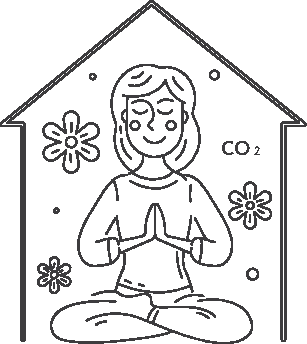
\includegraphics[scale=1.5]{willpower/ch11/6.pdf}
\end{figure}

\textbf{Праблема вэнтыляцыі} існуе: з~аднаго боку, будаўнікі часта грэбуюць нормамі, робячы няўдалыя сыстэмы вэнтыляцыі, эфэктыўнасьць работы якіх ніхто не правярае. Зь цягам часу шахты могуць забівацца брудам, зашывацца~--- звонку гэта не прыкметна. Зьяўленьне плястыкавых вокнаў яшчэ пагоршыла сытуацыю. Бо ў~драўляных вокнах было шмат невялікіх шчылінаў, якія забясьпечвалі мікравэнтыляцыю, а~цяпер гэтага няма. Часта мы закрываемся ``наглуха'' для цішыні або цяпла. Зьяўленьне ізалявальных матэрыялаў, ушчыльняльнікаў, пракладак для дзьвярэй і вокнаў дазваляе нам цалкам зашпунтаваць сябе ў~хатах. А калі прытоку паветра няма, то і вэнтыляцыя перастае працаваць як мае быць.

\textbf{Перадусім~--- вымяраем!} Існуе вялікая колькасьць датчыкаў, як аўтаномных, так і такіх, што сынхранізуюцца са смартфонамі. Хоць мы вымяраем узровень вуглякіслага газу, гэтая лічба кажа нам і аб якасьці вэнтыляцыі ў~цэлым. Чым менш узровень CO\textsubscript{2}, тым лепш якасьць паветра, уключаючы разнастайную колькасьць выдыханых намі малекул і нават бактэрыяў. CO\textsubscript{2} выступае як газ-дэтэктар якасьці паветра.

\textbf{Ідэальныя ўзроўні CO\textsubscript{2}~--- да 450 ppm, прымальна да 600--800, стандартная норма да 1000, ад 1000 да 2500~--- млявасьць, зьніжэньне самаадчуваньня, дрэнны сон і да т.~п., вышэй за 2500 ppm~--- пажадана пакінуць памяшканьне.}

Высокі ўзровень CO\textsubscript{2} уплывае на тонус сасудаў галаўнога мозгу, зьніжае прадуктыўнасьць, уважлівасьць і ініцыятыўнасьць. Яго высокія ўзроўні непажадана ўзьдзейнічаюць на мозг і цела, павялічваецца кіслотнасьць плазмы крыві, зьмяняецца тонус сасудаў. Павялічваецца частата галаўных боляў, рэзка падае прадуктыўнасьць, пагаршаецца памяць і шматлікія паказьнікі мысьленьня, асабліва ў~рашэньні складаных задач. Чым менш пакой, больш у~ім людзей~--- тым вышэй узровень CO\textsubscript{2}.

Акрамя мозгу, растуць рызыкі для цела. Напрыклад, павялічваецца ўзровень запаленьня праз актывацыю NLRP3 інфламасомаў і павышэньне ўзроўню IL-1β, узмацняецца пульс спакою, павышаецца рызыка дэпрэсіі. Цікава, што гіпэркапнія і зьніжэньне pH плазмы стымулюе арэксінавыя нэўроны і ўзмацняе апэтыт! Ёсьць дасьледаваньні аб тым, што гіпэркапнія непасрэдна стымулюе рост тлушчавых клетак. Таксама пры працяглыях падвышаных узроўнях вуглякіслага газу вышэй рызыка саркапэніі, астэапарозу, хранічных хваробаў нырак. Высокія ўзроўні вуглякіслага газу 2,000~--- 3,000 ppm узмацняюць кальцыфікацыю нырак і паскараюць дэмінэралізацыю костак.

Асабліва небясьпечна гэта ў~офісах, дзе ў~адным памяшканьні можа адначасова знаходзіцца вялікая колькасьць людзей. У школах узровень CO\textsubscript{2} вышэйшы за 1000 ppm у~некалькі разоў павялічваў захворваньне на ВРЗ. Узмацняецца выдзяленьне вуглякіслага газу пры занятках спортам, а~калі спартзаля не абсталяваная адэкватнай вэнтыляцыяй, гэта можа нэгатыўна паўплываць на здароўе спартоўцаў.

Чым больш людзей, тым інтэнсіўнейшая патрабуецца вэнтыляцыя для падтрыманьня нармальнай канцэнтрацыі вуглякіслага газу. Выбірайце памяшканьні зь вялікім аб'ёмам, каб вам заўсёды ставала, чым дыхаць. Пры куплі жыльля пажадана лічыць ня толькі квадратныя мэтры, але і кубічныя. Гэх, я так люблю высокія столі! Памятайце, што кандыцыянэр забясьпечвае астуджэньне паветра, ганяючы адзін і той жа яго аб'ём, таму без прытоку сьвежага паветра будзе назапашвацца вуглякіслы газ.

\textbf{Прыток і адток паветра.} Неабходна забясьпечыць як прыток паветра, так і яго адток. Пры адсутнасьці аднаго ці іншага якасьць вэнтыляцыі падае. Эфэктыўнасьць выцяжкі праверыць лёгка~--- запаліце запалку і патушыце, дым ад яе павінен уцягвацца ў~адтуліну. У ідэале сіла выцяжкі павінна быць такой, каб утрымліваць аркуш паперы.

\infobox{Ветраньне дома дапамагае хутка ачысьціць паветра, але пры закрытых вокнах і адсутнасьці выцяжкі вуглякіслы газ за пару гадзінаў зноў назапасіцца да небясьпечных узроўняў.}

На жаль, проста адкрыць вокны не заўсёды магчыма, бо гэта астуджае кватэру, упускае шум, праз адкрытыя вокны паступае паветра без папярэдняй ачысткі.

Па меры павелічэньня эфэктыўнасьці прытоку паветра ў~хаце важна зрабіць: прытокавыя клапаны пасіўныя, затым прытокавая прымусовая вэнтыляцыя з~ачысткай паветра, прытокавая-выцяжная вэнтыляцыя з~CO\textsubscript{2}-датчыкам, якая падтрымлівае дакладны ўзровень CO\textsubscript{2} у~залежнасьці ад колькасьці людзей у~памяшканьні і дазваляе эканоміць электрычнасьць і цеплыню, калі ў~пакоі нікога няма. Для эканоміі цяпла ёсьць адмысловыя сыстэмы рэкупэрацыі. Вядома, такія сыстэмы дарагія, палепшыць сытуацыю дапамагаюць і простыя пасіўныя прытокавыя клапаны і прачыстка вэнтыляцыйных шахт, усталёўка ў~іх прымусовай выцяжкі. Зьніжэньне ўзроўню CO\textsubscript{2} зьніжае колькасьць лятучых арганічных злучэньняў, фармальдэгіду, колькасьць бактэрыяў і грыбкоў у~паветры.

\subsection*{Пытаньні і заданьні}

1. Вымерайце ўзровень вуглякіслага газу дома ў~дзённы і вячэрні час.

2. Праверце працу выцяжных шахтаў у~вас у~хаце. Ці дастатковая ў~іх цяга?

3. Пры неабходнасьці, усталюйце пасіўныя або актыўныя сыстэмы прытоку паветра.


\section{Шум}

Шум не раздражняе адно тады, калі ты ў~ім удзельнічаеш~--- так кажуць, і гэта праўда. Сярод стрэсагенных чыньнікаў для насельнікаў кватэр шум упэўнена займае адно зь першых месцаў. Сваю кватэру, дзе я цяпер пішу гэтыя радкі, я абраў, у~тым ліку, па крытэры цішыні~--- верхні паверх, вуглавая кватэра і вокны на тры бакі, стары цагляны дом. Прымусіў мяне гэта зрабіць няўдалы папярэдні досьвед з~шумнымі суседзямі. 

\emph{Выдатна разумею фразу гішпанскага пісьменьніка Рамона Сэрна, што ``ўключаны пыласос у~суседа ўцягвае ўсе нашы думкі''.}

Чаму ж так цяжка прыстасавацца да шуму? Бо мы рэагуем на яго вельмі хутка. Гук~--- гэта адна з~крыніц інфармацыі аб навакольным сьвеце. Нас атачаюць гукі, як прыемныя прыродныя: птушкі, хвалі, дождж, так і небясьпечныя: гук стоенага злодзея або выбух пэтардаў. Асаблівасьць у~тым, што мы рэагуем на гукавыя раздражняльнікі хутчэй, чым на візуальныя, 140--160 мілісэкунд супраць 180--200, таму цяжэй тармазіць сваё раздражненьне.

\infobox{Запуск стрэсавай рэакцыі на нязвыклы гук, які перавышае звычайны фон,~--- гэта старажытны эвалюцыйны мэханізм выжываньня.}

Да шумавога забруджваньня, як і да сьпёртага паветра, можна звыкнуць і перастаць заўважаць, але вось псыхалягічнае прывыканьне не суправаджаецца фізычным.

\emph{Клясычны прыклад уплыву шуму~--- гэта гісторыя публічнай школы 98 у~Мангэтэне, дзе шум ад чыгункі стаў перашкаджаць дзецям вучыцца. Пра гэта даведалася псыхоляг Арлін Бронзафт і вывучыла сытуацыю. Аказалася, што ў~тым крыле школы, якое выходзіць вокнамі на пуці, шум прывёў да адставаньня ў~пасьпяховасьці на 11 месяцаў у~параўнаньні з~аднагодкамі ў~ціхім крыле школы. Шум перашкаджаў чуць, адцягваў увагу, настаўнікі былі вымушаныя павышаць голас. Сіла ведаў вялікая~--- пасьля апублікаваньня вынікаў і грамадзкай дыскусіі ўлады ўстанавілі спэцыяльныя гумовыя супрацьшумавыя пракладкі паміж шпаламі і рэйкамі каля школы. Шум зьнізіўся ўсяго на 8 дб, але гэтага было дастаткова, каб празь некалькі месяцаў адрозьненьні ў~пасьпяховасьці зьніклі.}

Самы небясьпечны хранічны стрэс~--- гэта той, якога мы не заўважаем: нязручнае крэсла прыводзіць да гіпадынаміі, сіні экран увечары зьбівае біярытмы, начны шум мы ігнаруем, калі ён не замінае спаць. Гэта распаўсюджаная і небясьпечная памылка: «Калі я не прачынаюся ад шуму, то ён не небясьпечны». На жаль, гэта ня так. Падчас сну слыхавая сыстэма працягвае функцыянаваць, і фізыялягічныя рэакцыі не адаптуюцца нават празь месяцы і гады начнога шуму: гэта скокі пульсу, выкід адрэналіну, парушэньне фазаў сну ды іншыя стрэсавыя рэакцыі. Вы можаце не высыпацца, бо ваш сон праз шум фрагмэнтуецца, і ў~выніку мы маем карціну недасыпу пры нармальнай колькасьці гадзінаў сну.

\emph{Начны шум~--- гэта нябачная крыніца хранічнага стрэсу, які назапашваецца. Ён выклікае эндатэліяльную дысфункцыю (пашыральнасьць артэрый), павялічвае аксідатыўны стрэс, пагаршае імунітэт і павялічвае ціск. У шэрагу дасьледаваньняў паказана залежнасьць частаты артэрыяльнай гіпэртэнзіі ад ажыўленасьці вуліцы, куды выходзяць вокны спальні: калі на дарогу, рызыка значна вышэйшая. Яшчэ вышэйшая рызыка ў~тых, хто сьпіць з~адкрытымі вокнамі, якія выходзяць на дарогу.}

\textbf{Цішыня на вагу золата.} Чым вышэйшая шчыльнасьць насельніцтва і больш мэханізмаў вакол нас, тым больш і шуму. У сучасным сьвеце, калі шчыльнасьць насельніцтва ўзрастае, шчыльнасьць забудовы расьце, колькасьць аўтамабіляў павялічваецца, зьяўляецца больш гукаўзнаўляльных прылад, шумных прыбораў і да т.~п., колькасьць шуму становіцца неймаверна вялікая ў~любы час содняў. Гэтая зьява атрымала назву ``шумавое забруджваньне''~--- па аналёгіі са сьветлавым, цеплавым, інфармацыйным.

\infobox{Цішыня цяпер становіцца рэсурсам, раскошай, за якую людзі гатовыя плаціць вялікія грошы.}

Больш за палову насельніцтва падвяргаюцца рэгулярнаму ўзьдзеяньню шуму вышэй за 55 дэцыбелаў (пры норме да 40). Асноўныя крыніцы шумавога забруджваньня~--- гэта транспарт (аўтамабілі, матацыклы, цягнікі, самалёты), забаўляльныя мерапрыемствы і кавярні, шум ад суседзяў. Часта ўнутры рэстарацыяў, ня кажучы ўжо пра клюбы, гук мацнейшы за норму.

Чым гэта небясьпечна? Шум адмоўна дзейнічае на многія сыстэмы, перш за ўсё на сардэчна-сасудзістую і нэрвовую. Сярод людзей, якія працуюць у~шумных умовах, прыкметна вышэй працэнт псыхічных парушэньняў. Шум павышае артэрыяльны ціск, вядзе да пастаяннага павышанага ўзроўню гармону стрэсу картызолу, пагаршае якасьць сну і можа прыводзіць да дрымотнасьці і няшчасных выпадкаў днём, бессані, атлусьценьня, гіпэртэнзіі, дэпрэсіі, парушэньня кагнітыўных здольнасьцяў, павышае рызыку інфаркту міякарда (ужо пры ўзроўні вышэй за 50дБ).

\textbf{Акустычны стрэс} можа назапашвацца. Калі ад шуму на працы можна аднавіцца дома, то шум з~раніцы да ночы наносіць узмоцненую шкоду здароўю. Самы ўразьлівы час~--- гэта моманты засынаньня і абуджэньня. Шум падчас засынаньня падаўжае пэрыяд адыходу да сну, замінае яму. Моцнае раздражненьне ад шуму зьвязанае яшчэ і з~асаблівасьцямі асобы пэўнага чалавека. Кагосьці больш ятрыць шум суседзяў, кагосьці~--- аўтамабіляў. Шум адымае вялікую колькасьць псыхічных рэсурсаў, бо павялічвае ўзрушанасьць і адцягвае, патрабуючы канцэнтрацыі ўвагі. Шум пагаршае прыняцьце рашэньняў і зьмяншае здольнасьць супраціўляцца стрэсу.

\textbf{Людзі з~наяўнымі псыхалягічнымі праблемамі, дэпрэсіяй могуць больш гостра рэагаваць на шум, чым астатнія.}

\emph{Пачынаючы з~узроўню 45 дБ, кожныя дадатковыя 5дБ павялічваюць акружнасьць таліі на 2 мм. Дзеці, якія растуць у~шуме, адстаюць ад аднагодкаў: кожныя 5дБ шуму дадаюць яшчэ 2 месяцы да таго моманту, як дзіця пачне чытаць. Пастаяннае ўзьдзеяньне інтэнсіўнага шуму (80 дБ і больш) можа стаць прычынай гастрыту і нават язвавай хваробы, бо могуць парушацца сакраторная і маторная функцыі страўніка.}

Адно з~дасьледаваньняў паказала, што жыхары вёскі, над якой пралятаюць самалёты, часьцей зьвяртаюцца да лекара, чым жыхары вёсак, разьмешчаных убаку ад авіямаршрутаў. Галоўнай крыніцай гарадзкога, то бок вонкавага шуму часьцей за ўсё зьяўляецца аўтатранспарт~--- больш за 60\,\% скаргаў на шум жыхароў усяго сьвету зьвязаныя менавіта з~аўтамабілямі і грамадзкім транспартам.

Гукі ўплываюць на нас і больш тонкімі мэханізмамі, мяняючы наша ўспрыманьне рэальнасьці. Напрыклад, француская музыка ў~краме павялічвае імавернасьць таго, што вы купіце францускае віно. Гучная музыка аслабляе ўспрыманьне салодкага і салёнага, што можа правакаваць пераяданьне. Таму важна есьці пад прыемную і нягучную музыку. Часьцей слухайце любімыя песьні і мэлёдыі~--- гэта выдатная антыстрэсавая мэтодыка.

\subsection*{Пытаньні і заданьні}

1. Вымерайце ўзровень шуму на працы і дома. Ці перавышае ён норму?

2. Ці замінае шум вам засыпаць? Ці прачынаецеся вы ад шуму?

3. Вам лягчэй працаваць у~цішыні ці фонавы шум вам дапамагае?


\section{Як змагацца з~шумам}

Самая эфэктыўная мера~--- гэта заканадаўчыя абмежаваньні ды іх выкананьне. Забараняюцца самыя розныя крыніцы шуму, так, у~XVI стагоддзі каралева Брытаніі Лізавета забараніла скандалы і сямейныя сваркі пасьля 22:00, а~ў Швайцарыі і сёньня забаронена пасьля 22:00 карыстацца душам і прыбіральняй. Вы можаце выступіць за ціхую гадзіну ў~вашым доме, прагаласаваць за выкарыстаньне шумапаглынальных пакрыцьцяў у~месцах агульнага карыстаньня, забарону праслухоўваньня гучнай музыкі і да т.~п. Зялёныя зоны ў~горадзе і павелічэньне колькасьці электратранспарту памяншаюць колькасьць шуму.

Зьмены ў~рамках кватэры варта пачаць з~вымярэньня шуму і выяўленьня яго асноўных крыніц. Замерайце ўзровень шуму ў~асобных памяшканьнях: ваш працоўны габінэт, спальня, дзіцячы пакой. Для гэтага можна выкарыстоўваць адмысловыя праграмы, напрыклад SoundPrint, IHearU або NoiseTube~--- яны ператвараюць смартфон у~шумамер. Вызначыце асноўныя крыніцы шуму ў~вашай кватэры: суседзі, адкрытыя вокны, гучныя электрапрыборы?

\emph{Для мяне ўзровень шуму~--- гэта адзін з~найважнейшых крытэрыяў выбару жыльля: удалечыні ад буйной дарогі, з~вокнамі ў~двор, зь мінімальнай колькасьцю кантактаў з~суседнімі кватэрамі.}

Калі вы плянуеце рамонт, то загадзя вымярайце гукаізаляцыю сьценаў і, калі ёсьць неабходнасьць, плянуйце яе ўсталёўку. Ёсьць шмат розных падыходаў: вібрападвесная столь, спэцыяльная гукаізаляцыя падлогі і сьценаў, шумапаглынальныя дзьверы, шматкамэрныя шклопакеты, прытокавая вэнтыляцыя. Максімальная лічба, на якую здольныя паменшыць шум шматслаёвыя канструкцыі,~--- 15 дБ. Практычна гэта мяжа для дадатковай гукаізаляцыі існых сьценаў і перакрыцьцяў. Памятайце пра неабходнасьць гукаізаляцыі камунікацый (паветраводы і трубы, інжынернае абсталяваньне), а~таксама «слабых месцаў», такіх як разэткі і дзьверы. Купляйце бытавую тэхніку (лядоўню, кандыцыянэр) зь нізкім узроўнем шуму, ён пазначаны ў~апісаньні прыбораў.

Калі мы вядзём гаворку пра памяшканьне, важна ўлічваць і акустычны камфорт, які парушаецца залішнім адлюстраваньнем гуку, што значна павялічвае зашумленасьць памяшканьня. Пры гэтым староньнія шумы змушаюць увесь час напружваць слых і падвышаць голас. Паляпшэньне акустычнага камфорту мяркуе стварэньне гукапаглынальных паверхняў: калі сьцены і столь памяшканьня зробленыя зь цьвёрдых матэрыялаў, якія добра адбіваюць гук (напрыклад, з~гіпса-кардонных лістоў), то ў~памяшканьні будзе назірацца падвышаная гулкасьць. Стварэньне камфортнага асяродзьдзя вырашаецца з~дапамогай выкарыстаньня ў~інтэр'еры памяшканьняў дэкаратыўных акустычных панэляў. Сэнсу дабівацца поўнай цішыні няма, яна можа быць нават некамфортная для чалавека.

\begin{figure}[htb!]
  \centering
  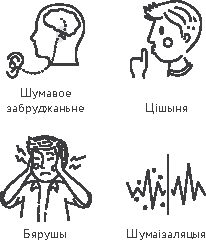
\includegraphics[scale=1.5]{willpower/ch11/7.pdf}
\end{figure}

\textbf{Навушнікі і бярушы.} Бярушы~--- старажытнае вынаходства, ім некалькі тысячаў гадоў: яшчэ Адысэй заляпіў воскам вушы сваёй камандзе, каб яны не паддаліся песьням сырэнаў і не разьбілі аб скалы карабель. Бярушы~--- гэта просты, танны і вельмі эфэктыўны спосаб барацьбы з~шумам. Цікава, але яны паляпшаюць сон нават у~тых людзей, хто ўпэўнены, што гукі ім не замінаюць. Я сам даўно карыстаюся бярушамі і вельмі шаную іх ахоўнае дзеяньне на мой сон і нэрвы. Бярушы дапамагаюць адпачыць у~транспарце, ноччу, калі ў~вас маленькія дзеці або гучныя суседзі. Асабліва гэта актуальна для людзей, якія адчуваюць стомленасьць ад шуму або маюць павышаную да яго адчувальнасьць.

\emph{Ёсьць шмат відаў бярушаў: гумовыя, сіліконавыя, васковыя і да т.~п. Я аддаю перавагу васковым, бо яны разьмякчаюцца і прымаюць форму слыхавога праходу, ня ціснуць на ягоныя сьценкі, у~адрозьненьне ад паралёнавых. Для самых прасунутых ёсьць індывідуальныя бярушы, якія могуць вырабіць са зьлепку вуха.}

Яшчэ адным спосабам абароны вушэй, прыдатным для паўсядзённай працы, зьяўляюцца шумавыя фільтры, якія выбарча адсякаюць толькі гучныя гукі, пакідаючы спэктар чалавечага голасу. Такімі бярушамі ці навушнікамі можна карыстацца на вуліцы, у~мэтро ці ў~самалёце, а~таксама працуючы сярод шуму. Цяпер шмат навушнікаў з~функцыяй шумапрыглушэньня, якая счытвае гук звонку і памяншае яго, транслюючы ўнутр у~супрацьфазе.

\textbf{Выкарыстоўвайце белы і ружовы шум.} Адна з~карысных уласьцівасьцяў белага шуму~--- ствараць тло, якое маскіруе іншыя гукі. Бо найболей непрыемным для сну ці канцэнтрацыі ўвагі зьяўляецца ня сам гук, а~рэзкая зьмена гукавога тла. Наадварот, шматлікія прыродныя гукі, такія як шолах ветру, шум хваляў ці дажджу, валодаюць карыснымі эфэктамі. Белы гук рэкамэндуюць для палягчэньня засынаньня дзяцей, для лепшай канцэнтрацыі, ён эфэктыўны для людзей з~тынітусам (звон у~вушах), паляпшае якасьць і глыбіню сну, дапамагае склейваць фрагмэнты сну.

\textbf{Аднак белы шум высокай гучнасьці можа быць шкодны для мозгу, асабліва для мозгу маленькіх дзяцей, таму варта выкарыстоўваць яго зь нізкай гучнасьцю і не на настаяннай аснове.}

Акрамя белага шуму, ёсьць і шэраг іншых, ад ружовага да карычневага. Калі белы шум мае роўную інтэнсіўнасьць на ўсіх частотах, то спэктральная шчыльнасьць ружовага шуму памяншаецца з~павелічэньнем частаты, і ён таксама выдатна маскіруе гукі. Белы і ружовы шумы выкарыстоўваюць у~офісах, што дазваляе павысіць канцэнтрацыю і памяць, зьнізіць адцягвальнасьць. Ружовы шум у~дасьледаваньнях дапамагае палепшыць фазу глыбокага сну ў~пажылых пацыентаў і вынікі кагнітыўных тэстаў. Адсотак памылак пры працы пад ружовы шум не нашмат вышэйшы, чым пры працы ў~поўнай цішыні.

\emph{Вы можаце знайсьці на Youtube разнастайныя запісы шумоў ці гукаў прыроды.}

\textbf{Музыка і прадуктыўнасьць.} Многім людзям музыка дапамагае сфакусавацца і больш прадуктыўна працаваць. Унівэрсальных рэкамэндацыяў тут няма, галоўнае~--- кіравацца асабістымі перавагамі і экспэрымэнтаваць. У ідэале тып музыкі мусіць адпавядаць тыпу вашае працы. Музыка можа матываваць і паляпшаць агульны настрой. Многім дапамагаюць мэлёдыі для рэляксу, клясычная музыка і да т.~п.

\textbf{Насалоджвайцеся цішынёй.} Цішыня мае тэрапэўтычнае значэньне і зьяўляецца рэсурсам: практыка маўчаньня і захаваньня цішыні распаўсюджаная ў~розных духоўных традыцыях. На Усходзе практыка маўчаньня называецца ``маума'', Махатма Гандзі прысьвячаў ёй дзень на тыдзень.

\emph{У горадзе, дзе я вырас, быў манастыр манахаў картэзіянцаў, якія шырока выкарыстоўвалі практыку маўчаньня. Зьняты пра іх жыцьцё фільм так і называўся~--- ``Вялікае бязмоўе''.}

Практыка маўчаньня ўключае як адмову ад маўленьня, так і адсутнасьць шумнага асяродзьдзя, а~таксама~--- ``цішыню розуму''. Цяпер шматлікія з~нас пачуваюцца ў~цішыні некамфортна і імкнуцца заглушыць яе радыё ці тэлевізарам, у~гутарцы зь іншымі мы пазьбягаем паўзаў, запаўняючы іх пустой балбатнёй.

\infobox{Устрыманасьць ад пустых размоваў, ныцьця, крытыкі, скаргаў, парадаў~--- усё гэта трэніруе ўвагу і робіць маўленьне мацнейшым і выразьнейшым.}

Дасьледаваньні пацьвярджаюць, што дзьве гадзіны поўнай цішыні могуць стымуляваць нэўрагенэз у~гіпакампе і палепшыць кагнітыўныя здольнасьці. Пэрыядычна рабіце «ціхі час» у~офісе~--- устрыманьне ад размоваў і перапіскі~--- гэта дапаможа павысіць прадуктыўнасьць. Дадайце ў~свой дзень моманты цішыні між працай і сустрэчамі, бо, як слушна заўважыў Барыс Пастарнак, ``цішыня~--- ты найлепшае з~таго, што я чуў''.

\subsection*{Пытаньні і заданьні}

1. Ці адчуваеце вы ўзьдзеяньне акустычнага стрэсу?

2. Паэкспэрымэнтуйце зь бярушамі. Як цішыня ўплывае на вашую працоўную прадуктыўнасьць, на якасьць сну?

3. Падумайце, як можна аптымізаваць вашае жыльлё для зьніжэньня ўзроўню шумавога забруджваньня з~вонкавых і ўнутраных крыніцаў?


\section{Хворы дом~--- хворыя жыхары}

\emph{Калі мы разглядаем старадаўнія карціны віктарыянскай эпохі, то ўвагу, апроч іншага, прыцягвае яркі зялёны колер сьценаў і ярка-зялёнае адзеньне. Сама каралева Вікторыя любіла смарагдава-зялёныя сукенкі, чым задала моду сярод сваіх падначаленых. Гэтая фарба адценьня «парыская зеляніна» ў~сваёй аснове ўтрымлівала мыш'як, і ёю фарбавалі сьцены, тканіны, цацкі. Такія «зялёныя» дамы падрывалі здароўе сваіх жыхароў і выклікалі цяжкія атручэньні, у~тым ліку і са сьмяротным зыходам. Толькі праз сто гадоў выкарыстаньня гэтага фарбавальніка яго шкоду ўсьвядомілі ў~поўнай меры і замянілі бясьпечнымі аналягамі.}

Сучасныя рэаліі такія, што больш за 90\,\% свайго часу чалавек праводзіць у~памяшканьні. Гэтаму спрыяюць узмацненьне урбанізацыі, ушчыльненьне гарадоў і пагаршэньне гарадзкога асяродзьдзя. На жаль, гарады часта робяцца ўсё больш небясьпечнымі для фізычнага, псыхалягічнага і сацыяльнага здароўя, таму дом становіцца крэпасьцю, сховішчам і месцам адпачынку. З павелічэньнем колькасьці людзей, якія працуюць дыстанцыённа, дом становіцца офісам, спартзаляй, канцэртнай заляй, студыяй, рэстарацыяй і гэтак далей. Разьвіцьцё інтэрнэт-тэхналёгіяў імкліва скарачае неабходнасьць пакідаць кватэру. Таму ўплыў хатняга асяродзьдзя на здароўе заслугоўвае пільнай увагі.

Калі я пішу гэтыя радкі, амаль палова чалавецтва закрытая ў~лакдаўне ў~сваіх дамах праз ковід, што прымушае па-новаму пераасэнсаваць бясьпеку сваёй хаты. Бо здароўе гаспадароў залежыць ад здароўя іх дома!

\textbf{Сындром хворага будынка.} Ужо больш за сто гадоў існуе тэрмін «сындром хворага будынка»~--- калі выяўляецца прамая прычынна-выніковая сувязь паміж станам здароўя і пражываньнем у~канкрэтным памяшканьні. Шэраг дасьледаваньняў паказвае, што каля 30\,\% будынкаў шкодзяць здароўю сваіх насельнікаў. Рэдка ўдаецца знайсьці адну-адзіную прычыну праблемаў~--- гэта зьвязана з~тым, што сымптомы разладу здароўя ў~людзей узьнікаюць пры знаходжаньні ў~памяшканьнях, дзе парамэтры асяродзьдзя не перавышаюць агульнапрынятых гранічна дапушчальных канцэнтрацыяў. Найбольш імавернай прычынай гэтага зьяўляецца эфэкт узаемнага патэнцыяваньня дзеяньня дзясяткаў розных рэчываў у~паветры памяшканьняў.

Усе нэгатыўныя чыньнікі можна падзяліць на дзьве групы:

1. \textbf{Нездаровы мікраклімат.} Гэта адмоўна дзейсныя нэгатыўныя фактары мікраклімату: вільготнасьць, тэмпэратура, сьвятло і інш. Іх лішак ці недахоп у~пэўных умовах можа нэгатыўна адбівацца на здароўе. Асобна варта разгледзець мікраклімат дома, яго ўборку, вэнтыляцыю і наяўнасьць шкодных злучэньняў. Усе гэтыя чыньнікі могуць узаемадзейнічаць паміж сабой.

2. \textbf{Прамыя пашкоджвальныя чыньнікі.} З магчымых пашкоджвальных чыньнікаў можна назваць лішак вуглякіслага газу, электрасмог (інтэнсіўнае электрамагнітнае выпраменьваньне), алергенныя чыньнікі: зароднікі цьвілі, фэкаліі хатніх кляшчоў, сынтэтычныя раздражняльнікі (дробныя часьціцы плястыку і інш.), хімічныя рэчывы (часьцей за ўсё фэнол і фармальдэгід) і мноства іншых. Сам будынак, мэбля, абслугоўвальныя сыстэмы выдзяляюць небясьпечныя для здароўя рэчывы.

\emph{Аналіз паказвае, што ў~паветры жылых памяшканьняў і офісаў можа адначасова прысутнічаць больш за сотню хімічных злучэньняў, якія часта ў~некалькі разоў перавышаюць гранічна дапушчальныя канцэнтрацыі. Сярод іх~--- часьціцы волава, кадмію, ртуці, медзі, цынку, фэнолу, фармальдэгіду, таксічныя выпарэньні ад мыйных і чысьцільных сродкаў і інш.}

\begin{figure}[htb!]
  \centering
  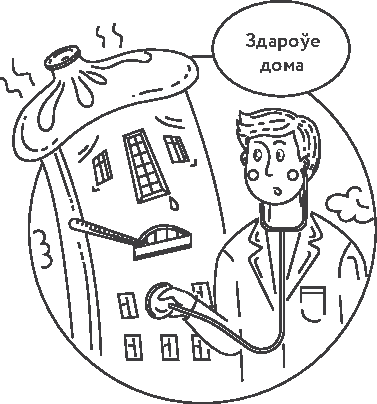
\includegraphics[scale=1.2]{willpower/ch11/8.pdf}
\end{figure}

У памяшканьнях паветра бруднейшае, чым на вуліцы, канцэнтрацыя ўнутры можа быць у~сотні разоў вышэй, чым на адкрытым паветры. Пыл, часьціцы якога нябачныя для вока, практычна не асядае, увесь час вісіць у~паветры і зьяўляецца адной з~асноўных крыніц інфэкцыяў: мікробы і бактэрыі выкарыстоўваюць яе часьціцы (памерам меней за 10\,мкм) для перасоўваньня і кантакту.

\infobox{Высокая вільготнасьць у~спалучэньні з~кепскай вэнтыляцыяй павялічвае рызыку зьяўленьня цьвілі, удыханьня зароднікаў, якія могуць быць шкоднымі для здароўя. Крыніцай забруджваньня паветра ў~памяшканьні можа стаць і занадта дбайная ўборка з~выкарыстаньнем вялікай колькасьці сродкаў бытавой хіміі.}

Праводзіць дома занадта вялікую колькасьць часу~--- гэта ня вельмі ўдалая ідэя. У хаце мы менш рухаемся, у~нас узьнікае дэфіцыт сонечнага сьвятла, зьбедненае візуальнае асяродзьдзе, мы больш ямо і схільныя больш ляжаць ды ізалявацца ад сацыяльных кантактаў. Ну і, зразумела, дамашняе асяродзьдзе можа быць ня занадта карысным. Так indoor~--- гэта значыць унутрыдомавы~--- лад жыцьця можа нэгатыўна ўплываць на нас.

Зрабіце ўсё магчымае, каб ваш дом стаў максімальна здаровым месцам, якое забясьпечвае аўтаномію і абарону ад агрэсіўнага гарадзкога асяродзьдзя, узнаўляе натуральнае асяродзьдзе жыцьця, падтрымлівае псыхалягічны камфорт, дае пачуцьцё бясьпекі і адлюстроўвае вашы індывідуальныя перавагі.

\textbf{Здаровы дом~--- гэта прытулак, схоўня, месца, дзе мы можам адпачываць і аднаўляць свае сілы ў~аптымальным для гэтага мікраатачэньні.}

\subsection*{Пытаньні і заданьні}

1. Ці лічыце вы свой дом бясьпечным для здароўя?

2. Як мяняецца ваша самаадчуваньне пры працяглым знаходжаньні ў~памяшканьнях?

3. Колькі часу вы праводзіце дома? На вуліцы? У іншых памяшканьнях?


\section{Пыл, кляшчы і цьвіль}

Варта страсянуць посцілку ў~сонечнае надвор'е, як паветра напаўняецца незьлічонымі часьціцамі пылу~--- гэта тое, чым мы дыхаем у~сябе дома. Пыл можа нашкодзіць нашай псыхіцы і ў~выпадку, калі сваякі і госьці няўхваляльна ківаюць галавой пры выглядзе пласта пылу, і нашаму арганізму~--- калі мы яе ўдыхаем. Сапраўды, «пылінка ня бачная, ды выесьць вочы». 

\infobox{Вылучаюць чатыры асноўныя крыніцы ўзьнікненьня пылу: жывёлы, людзі, разбурэньне матэрыялаў дома і прынесеныя з~вуліцы часьціцы.}

Вялікая колькасьць пылу~--- гэта тыповая праблема памяшканьняў. Рэгулярная ўборка і нізкі ўзровень пылу важныя для здароўя дома і яго жыхароў. У звычайнай кватэры ў~год утвараецца да 40 кіляграмаў пылу, прыкметная іх частка трапляе ў~нашы лёгкія. Бо за содні мы ўдыхаем да 12 тысячаў літраў паветра, а~ў кожным літры можа быць да 500 пылавых часьціц.

\emph{Пылавыя часьціцы могуць быць аэраалергенамі, сярод іх~--- пылавыя кляшчы ды іх фэкаліі, грыбы і іх зароднікі, прадукты жыцьцядзейнасьці сабакаў, катоў, прусакоў, пылок расьлінаў і інш. Гэта можа пашкоджваць сьлізістыя і павялічваць рызыку алергічных захворваньняў.}

Цьвіль расьце ў~вільготным асяродзьдзі, таму сачыце, каб узровень вільготнасьці ня быў занадта высокім. Важна правяраць і чысьціць асушальнікі і кандыцыянэры, інакш яны самі могуць стаць крыніцай бактэрыяльнага і грыбковага забруджваньня. Чысьціць фільтры ў~кандыцыянэры трэба мінімум раз на два месяцы і не забываць прыбіраць пыл з~самога прыбора. Цьвілёвасьць памяшканьняў можа павялічваць узровень хранічнага запаленьня.

Вялікае значэньне мае і ўплыў бактэрыяў. Напрыклад, пры залішняй вільготнасьці павялічваецца канцэнтрацыя бактэрыяў Streptomycetes і канцэнтрацыя выдзяляных ёю эндатаксінаў у~паветры. Высокая канцэнтрацыя эндатаксінаў у~паветры можа выклікаць разьвіцьцё недыху і рэўматычных захворваньняў. Абсалютная стэрыльнасьць жытла там таксама не патрэбная: доза бактэрыяў мае U-падобны ўплыў на здароўе. Пры нізкіх і сярэдніх узроўнях яна зьніжае рызыку алергій і недыху, а~вось пры высокіх~--- павышае.

Адэкватная вэнтыляцыя зьмяншае канцэнтрацыю бактэрыяў і вірусаў у~паветры. Гэта мінімізуе імавернасьць узьнікненьня інфэкцыяў, павялічвае прадукцыйнасьць працы супрацоўнікаў офісаў і пасьпяховасьць дзяцей у~школах. У дасьледаваньнях ультрафіялетавае абеззаражаньне (кварцаваньне) элемэнтаў ацяпленьня ў~офісах прыводзіла да зьніжэньня захворваньняў на ГРЗ.

\infobox{Абсалютная стэрыльнасьць жытла нам таксама не патрэбна: доза бактэрый мае U-вобразнае ўплыў на здароўі. Пры нізкіх і сярэдніх роўнях яна зьніжае рызыку алергій і астмы, а вось пры высокіх~--- павялічвае.}

\textbf{Не карміце кляшчоў.} Галоўная крыніца пылу і ежы для кляшчоў~--- гэта адпадкі эпітэлію нашай скуры, які назапашваецца, у~асноўным, у~пасьцельнай бялізьне. Таму трэба штотыдзень старанна яе праць пры тэмпэратуры 60° С і вышэй. Калі вы выкарыстоўваеце тэкстыльныя канапы, то не ляжыце на іх голым і ня сьпіце без прасьціны або замяніце іх на скураныя. Абмяжуйце колькасьць дзіцячых мяккіх цацак і рэгулярна іх мыйце.

\begin{figure}[htb!]
  \centering
  
\includegraphics[scale=1.5]{willpower/ch11/9.pdf}
\end{figure}

За сваё жыцьцё пылавы клешч вырабляе фэкаліяў у~2000 разоў больш, чым важыць сам, і менавіта яго адходы небясьпечнейшыя за ўсё. Кляшчы аддаюць перавагу цеплыні, вільгаць і эпітэлію скуры, таму нашы пасьцелі аптымальныя для іх жыцьцядзейнасьці і размнажэньня. Шмат іх можа быць у~тапках і падушках.

\subsection*{Цьвіль}

Самі па сабе цьвільныя грыбкі (любога кшталту: і бросьня на вадкасьцях, і плесьня~--- пушысты налёт на прадуктах, рэчах і рэштках) не выклікаюць інфэкцыяў~--- толькі ў~людзей з~сур'ёзным імунадэфіцытам. Але іх зароднікі і часьціцы, як жывыя, так і мёртвыя, у~высокіх канцэнтрацыях могуць выклікаць алергічныя рэакцыі і ўзмацняць запаленьне. Звычайна цьвіль аддае перавагу тэмпэратуры вышэй за 20 градусаў і вільготнасьці вышэй за 50. Дрэнны паветраабмен і кандэнсат на сьценах і мэблі (волкія і няветраныя памяшканьні) павялічваюць рызыку зьяўленьня цьвілі.

Цьвіль можа пасяліцца ў~сыстэмах апалу, кандыцыянэрах, пасудамыйных машынах, кветкавых гаршках, ванных, ня кажучы ўжо пра гарышчы і гаражы. Пазьбягайце працяглага знаходжаньня ў~такіх памяшканьнях, кантралюйце гідраізаляцыю, сачыце за сьценамі, дахам і камунікацыямі: у~іх не павінна быць працёкаў вады. Калі адна са сьценаў дома адсырэла, ня стаўце ўсутыч да яе мэблю. Высушвайце ручнікі, вяхоткі, сьмецьцевыя вёдры і не дазваляйце ім стаяць мокрымі доўгі час. Дбайнае ацяпленьне памяшканьняў зімой і восеньню памяншае рызыку цьвілі. Для апрацоўкі заражаных паверхняў выкарыстоўвайце спэцыяльныя супрацьплесьневыя сродкі, якія дазваляюць зьнішчыць яе на ўсёй глыбіні пранікненьня ў~матэрыял.

\subsection*{Як змагацца за чысьціню}

\textbf{Антыпылавы дызайн.} Арганізуйце сваю кватэру так, каб у~ёй назапашвалася менш пылу і яе было зручна прыбіраць. Пазбаўцеся ад дываноў і палавікоў або зьменшыце іх колькасьць~--- гэта самыя галоўныя пылазборнікі. Шторы ня толькі зацямняюць кватэру, але й зьбіраюць шмат пылу. Зрэшты, цяпер ужо зьявіліся ў~продажы запавесы, ачышчальныя ад пылу. Важна падтрымліваць вільготнасьць у~50--60\,\%~--- гэта перашкаджае залішняму ўтварэньню і распаўсюджваньню пылу: чым ніжэй вільготнасьць, тым больш будзе пылу. Адзеньне захоўвайце ў~закрытых шафах. Ідэальна захоўваць розныя статуэткі і кнігі ў~шафах за шклом. Прызнаюся, што нават мне гэта не ўдалося арганізаваць. Памятайце, што трэба рэгулярна адсоўваць мэблю і прыбіраць пылавыя пасткі, часта гэта месцы за батарэямі або на задняй сьценцы лядоўні.

\textbf{Здаровая прыборка.} Вільготная прыборка~--- важны складнік догляду за домам, ладзьце яе 1--2 разы на тыдзень. Звычайная вільготная прыборка выклікае прыкметнае скарачэньне мікрачасьціц пылу, і толькі праз тры дні іх колькасьць вяртаецца да ранейшага ўзроўню. Важна пазьбягаць выкарыстаньня хімічных мыйных сродкаў, лепш за ўсё ўжываць ачышчэньне парай і бясьпечнымі спосабамі, напрыклад вадой з~содай.

\emph{Устаноўлена, што ў~хатніх гаспадыняў, якія рэгулярна прыбіралі дом з~дапамогай хімічных мыйных сродкаў, на 40\,\% часьцей сустракаўся недых, у~параўнаньні з~тымі, хто іх не выкарыстоўваў.}

Заўсёды праводзіце прыборку зьверху ўніз, каб пазьбегнуць разносу пылу. Старадаўняя традыцыя выносіць рэчы на сонечнае сьвятло не пазбаўленая сэнсу. Рэч у~тым, што ўльтрафіялет ня толькі забівае кляшчоў, але й за пару гадзінаў раскладае іх алергены, чаго ня можа зрабіць нават кіпячэньне.

Калі мы пачынаем перабіраць кнігі ці пыльныя рэчы, то канцэнтрацыя пылу драматычна павялічваецца і можа дасягаць 1000 мг на кубамэтар паветра пры норме 10 мг. Мэханічнае ачышчэньне цьвілі ў~33 разы павялічвае канцэнтрацыю зароднікаў у~паветры.

\infobox{Прыбірайцеся ў~рэсьпіратары, дзяцей і ўвогуле сямейнікаў выпраўляйце на шпацыр на паўтары гадзіны, разнасьцежвайце вокны.}

Аптымальна выкарыстоўваць пыласосы з~НЕРА-фільтрамі, распрацаваныя адмыслова для алергікаў. Калі ў~вас ёсьць робат-пыласос, то можна запраграмаваць яго працу, калі вас няма дома і вокны адкрытыя. Так пыл, які ўздымаецца падчас прыборкі, не нашкодзіць вам. На жаль, большасьць звычайных пыласосаў толькі дробняць часьціцы пылу, а~чым драбнейшыя часьціцы, тым глыбей яны трапляюць у~лёгкія і мацней шкодзяць здароўю.

Паветраводы сыстэмаў прымусовага апалу і кандыцыянаваньні паветра могуць быць крыніцай забруджваньня ў~хаце. Калі ў~іх ёсьць цьвіль, скапленьне пылу і сьмецьця ці ў~паветраводах пасяліліся паразіты, неабходна тэлефанаваць прафэсіяналам, каб усё вычысьціць.

\begin{figure}[htb!]
  \centering
  
\includegraphics[scale=1.5]{willpower/ch11/10.pdf}
\end{figure}

\textbf{Выкарыстоўвайце фільтры.} Акрамя НЕРА-фільтраў, якія забясьпечваюць высокаэфэктыўнае затрыманьне часьціц, ёсьць фотакаталітычныя, газаачышчальныя, электрастатычныя, ультрафіялетавыя і іншыя тыпы фільтраў. Некаторыя вытворцы камбінуюць розныя прынцыпы ачысткі ў~адным прыборы. Эфэктыўнасьць працы фільтра трэба правяраць датчыкамі якасьці паветра.

\subsection*{Пытаньні і заданьні}

1. Як часта і якім чынам вы ладзіце прыборку?

2. Падумайце, што можна зьмяніць у~дызайне памяшканьня, каб там назапашвалася менш пылу і кляшчоў.

3. Падчас прыборкі праверце цяжкадаступныя месцы за шафамі, батарэямі, тэхнікай.


\section{Электрамагнітныя палі ды электрастатычная электрычнасьць}

У паветры лунае нешта нябачнае, што робіць шчасьлівымі ўсіх людзей. Пазбавіўшыся гэтага, людзі адчуваюць моцную пакуту і губляюць сэнс жыцьця. На жаль, гэта не флюіды любові, а~Wi-Fi і іншыя хвалі. Электрамагнітнае выпраменьваньне напаўняе нашае жыцьцё, але пытаньне яго ўзьдзеяньня на здароўе ўсё яшчэ вывучаецца.

\textbf{Электрасмог.} За апошні час у~нашых кватэрах зьявілася мноства прыладаў, якія генэруюць электрамагнітныя палі. Паасобку кожны з~прыбораў не небясьпечны, але сумарны іх уплыў (тэлефон, драды, імбрык, лядоўня, мультымедыя, ноўтбук, ЗВЧ-печка і інш.) выклікае асьцярогі ў~пляне ўплыву на здароўе. Электрасмог~--- гэта сукупнасьць электрамагнітных палёў, разнастайных частотаў, якія ўзьдзейнічаюць на чалавека ў~закрытых памяшканьнях.

У сапраўдны момант большасьць мэдыцынскіх супольнасьцяў лічыць узьдзеяньне электрамагнітнага выпраменьваньня бясьпечным. Ступень біялягічнага ўзьдзеяньня электрамагнітных палёў на арганізм чалавека залежыць ад частаты ваганьняў, напружанасьці і інтэнсіўнасьці поля, а~таксама працягласьці яго ўзьдзеяньня. Біялягічнае ўзьдзеяньне палёў розных дыяпазонаў неаднолькавае: паказаная шкода толькі вельмі высокіх яго значэньняў, таму жыць пад высакавольтнай лініяй перадач, вядома, небясьпечна.

\textbf{Ад выкарыстаньня тэлефона} назіраецца лякальнае павелічэньне тэмпэратуры, але малаверагодна, што гэта павялічвае рызыку раку. Адзінкавыя дасьледаваньні кажуць аб парушэньні выпрацоўкі мэлятаніну і зьніжэньні якасьці сну, але гэтыя дасьледаваньні назіральныя і не адлюстроўваюць прычынна-выніковай сувязі. Такім чынам, шкода ад электрамагнітнага выпраменьваньня тэлефона вельмі малая. 

\emph{Больш небясьпечнае няправільнае выкарыстаньне тэлефона, напрыклад, падчас кіраваньня аўтамабілем, у~тым ліку з~выкарыстаньнем гарнітуры. Гэта павялічвае рызыку дарожна-транспартных здарэньняў у~3--4 разы, але адбываецца праз страту ўвагі, а~не праз электрамагнітнае выпраменьваньне.}

Тым ня менш, па меры павелічэньня колькасьці прыбораў і інтэнсіўнасьці выпраменьваньня (укараненьне больш магутных 5G сетак і да т.~п.) важна захоўваць разумную засьцярогу і прытрымлівацца папераджальнай палітыкі, абмяжоўваць па меры магчымасьці залішняе ўзьдзеяньне электрамагнітных палёў.

\subsection*{Арганізуйце правільна праводку ў~доме}

Гэта ня толькі крыху паменшыць інтэнсіўнасьць поля, але й зьнізіць рызыку электратраўмы~--- хай усе разэткі будуць з~зазямленьнем. Сачыце, каб відэльцы шчыльна ўваходзілі ў~разэткі, а~прыборы былі спраўныя. Праводка ў~сьцяне не павінна праходзіць каля галавы, калі вы сьпіце (або лінія мусіць быць абясточаная).

\begin{figure}[htb!]
  \centering
  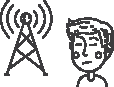
\includegraphics[scale=1.5]{willpower/ch11/11.pdf}
\end{figure}

\infobox{Ідэальным варыянтам зьяўляецца выкарыстаньне адмысловых выключальнікаў: калі ўсе прылады выключаны, то сетка ў пакоі адключаецца.}

\textbf{Абарона адлегласьцю.} Трымайце дыстанцыю: пры аддаленьні ад крыніцы электрычнага поля на падвойную адлегласьць напружанасьць поля зьніжаецца ў~4 разы. Пры аддаленьні на патройную адлегласьць велічыня поля зьніжаецца ў~9 разоў і г.~д. Калі працуеце, не трымайце на стале шмат уключаных у~сетку прыбораў. Адлегласьць у~паўмэтра ад звычайнай праводкі напраўду эфэктыўная.

\emph{Датчыкі электрамагнітнага поля каштуюць нядорага, зь іх дапамогай вы можаце самастойна вывучыць абстаноўку ў~вашай кватэры і рэальны ўплыў на яе прыбораў. Вымераць інтэнсіўнасьць палёў можна з~дапамогай Е-meter.}

Выключайце Wi-Fi на ноч, ня сьпіце ля праводкі і ўключаных прыбораў, абмяжуйце колькасьць «разумнай» тэхнікі, якая патрабуе падлучэньня да інтэрнэту і пастаяннага ўключэньня ў~сетку. Нават калі меры і не зьмяншаюць і без таго вельмі нізкую рызыку ад электрамагнітных палёў, гэта будзе карысна з~іншых прычынаў: эканомія энэргіі, прыбіраньне сьвятла ад індыкатараў тэхнікі ўначы і да т.~п.

\textbf{Электрастатычная электрычнасьць.} Яна ўзьнікае пры кантакце нашага цела з~рознымі паверхнямі: калі вы здымаеце ваўняны швэдар або расчэсваеце валасы сынтэтычнай расчоскай, ваша цела «электрызуецца». Скапленьне электрастатычнай электрычнасьці павялічвае назапашваньне пылу, а~вось нармальная вільготнасьць спрыяе расьсейваньню залішняга зараду.

\infobox{Бытавыя значэньні электрамагнітнага поля не паказалі значнага ўплыву на здароўе.}

У мінулым людзі ўвесь час кантактавалі зь зямлёй. Але цяпер мы ізалюем сябе штучнымі матэрыяламі, ад лінолеўму і лямінату да полівінілхлярыдных вырабаў, што прыводзіць да назапашваньня залішняга электрастатычнага зараду. Гэта яшчэ адзін сур'ёзны аргумэнт на карысьць клясычных натуральных матэрыялаў для будаўніцтва і рамонту. Існуюць адмысловыя антыстатычныя дабаўкі ў~лякі і фарбы, якія расьсейваюць электрычнасьць і не зьбіраюць пыл. Можна зазямляць мэблю, трубы.

\emph{Шырокі выбор антыстатычных кілімкоў, якія падключаюцца да гнёздаў вузла зазямленьня, пры гэтым можна мантаваць любыя паверхні, толькі важна іх правільна зазямляць. Праўда, практычная каштоўнасьць і навуковая абгрунтаванасьць гэтых падыходаў сумнеўныя.}

Падчас сну мы не ляжым нерухома ўвесь час, а~пэрыядычна рухаемся. Большасьць сынтэтычных вырабаў лёгка электрызуюцца, насычаючыся электрастатычнымі зарадамі, пры гэтым яны іх слаба расьсейваюць. Гэта вядзе да назапашваньня зараду на целе, што можа адмоўна ўплываць на наша самаадчуваньне. Акрамя гэтага, зарады пэрыядычна разраджаюцца, што парушае наш сон. Выбірайце пасьцельную бялізну з~натуральнае тканіны, якая не назапашвае лішні зарад; таксама сытуацыю паляпшае хаджэньне басанож увечары і водныя працэдуры.

\subsection*{Пытаньні і заданьні}

1. Ці шмат дратоў пад напругай і тэхнікі ля вашай галавы, калі вы сьпіце?

2. Праверце сваю праводку. Ці правільна падключаная і заземленая тэхніка?

3. Не насіце тэлефон у~кішэні і карыстайцеся гарнітурай для доўгіх размоваў.


\section{Вільготнасьць паветра}

\textbf{Просты ўплыў вільготнасьці.} Чым менш вільготнасьць паветра, тым мацней выпарэньне са скуры й сьлізістых абалонак.
Вільготнасьць паветра~--- важны складнік здаровага і камфортнага мікраклімату. Камфортнай лічыцца вільготнасьць ад 40\,\% да 60\,\%, прычым для высокіх тэмпэратураў (больш за 30°) трэба імкнуцца да вільготнасьці 30--50\,\%, пры тэмпэратурах менш за 20° C, наадварот, камфортнай будзе вільготнасьць 50--70\,\%. Пры больш высокай вільготнасьці мы лепей пераносім нізкія тэмпэратуры, а~пры нізкай~--- горай.

\subsection*{Нэгатыўны ўплыў падвышанай вільготнасьці}

Вялікая канцэнтрацыя вільгаці не дазваляе целу чалавека падтрымліваць звычайную тэмпэратуру~--- не працуе належным чынам мэханізм тэрмарэгуляцыі. Каб астудзіць сябе, чалавечае цела выкарыстоўвае потавыдзяленьне. Пот, выпараючыся з~паверхні скуры, выводзіць лішнюю цеплыню. Але што, калі выпарацца няма куды? Тады арганізм пачынае працаваць з~падвышанай сілай, а~гэта вядзе да зваротнага выніку~--- перагрэву. Калі пот зь цела выпараецца павольна, то цела астуджаецца вельмі слаба, і мы пачуваемся не зусім камфортна.

\emph{Асаблівае значэньне гэта мае для людзей, якія пакутуюць ад атэрасклерозу, гіпэртаніі, разнастайных захворваньняў сардэчна-сасудзістай сыстэмы,~--- яны мусяць быць асабліва асьцярожныя ў~сьпёку пры высокай вільготнасьці. Існуе магчымасьць рэзкага загостраньня захворваньняў і некантраляваных прыступаў.}

\textbf{Нэгатыўны ўплыў сухога паветра.} Чым ніжэй тэмпэратура паветра, тым менш у~ім утрымліваецца вады. Таму вонкавае паветра, які награецца батарэямі, мае нізкую адносную вільготнасьць. Зімой яе значэньне можа падаць да 20\,\%. А аптымальныя значэньні~--- 40--60\,\%. На наша здароўе вільготнасьць паветра аказвае прамы і непрамы ўплыў, давайце іх разьбяром.

\textbf{Прамы ўплыў вільготнасьці.} Чым менш вільготнасьць паветра, тым мацней выпарэньне са скуры і сьлізістых абалонак. У нашым носе і горле ёсьць тонкі пласт сьлізі, які абараняе нас ад трапляньня вірусаў, гэтая сьлізь увесь час абнаўляецца і перашкаджае перасыханьню. Калі паветра сухое на працягу доўгага часу, то ў~гэтай абароне ўтворацца расколіны, якія і зьяўляюцца ўваходнаю брамай для вірусаў.

\emph{Успомніце, як выглядае высахлая лужына ў~глінянай зямлі~--- яе дно пакрытае расколінамі.}

Перасыханьне сьлізістай дае нам нязручнасьць, таму мы кранаемся сьлізістай і тым самым пераносім вірус да «ўваходнае брамы».

І таму гэта павялічвае імавернасьць інфікаваньня~--- і сьлізісты бар'ер слабы, і самі перанесьлі вірус. Таксама сухасьць павялічвае колькасьць сымптомаў, зьвязаных з~абцяжараным дыханьнем, памяншае выпрацоўку сьлязы, павялічвае стомленасьць вачэй. Калі вы шмат гаворыце, то ваш голас хутчэй стоміцца і будзе горш гучаць у~сухім паветры. Таксама нізкая ці занадта высокая вільготнасьць уплывае на тэрмарэгуляцыю і якасьць сну.

\textbf{Непрамы ўплыў вільготнасьці.} Непрамы ўплыў вільготнасьці заключаецца ў~тым, як яна ўплывае на цыркуляцыю ў~паветры пылу і аэразоляў. Чым менш вільготнасьць, тым больш пылу і алергенаў знаходзіцца ў~паветры і тым даўжэй яны вісяць. Таму вільготнае паветра і чысьцейшае. У сухім паветры таксама запасіцца і больш электрастатычнай напругі. Вільготнасьць уплывае на выдзяленьне са сьценаў і матэрыялаў фармальдэгіду. У сухім паветры таксама даўжэй лётаюць аэразолі са зьмешчанымі ў~іх вірусамі і бактэрыямі. Стабільнасьць вірусу мінімальная пры 50\,\% вільготнасьці. Калі вільготнасьць 23\,\%, то ў~паветры 70--77\,\% вірусных часьціц, якія зьявіліся пры размове ці кашлі, а~вось пры вільготнасьці 43\,\% іх застаецца толькі 14\,\%. Гэта датычыцца і грыпу і каранавірусу.

Таксама сухое паветра вядзе да назапашваньня электрастатычнай электрычнасьці, назапашваньня пылу і павольнейшаму яе асяданьню. Мікрачасьціцы пылу яшчэ мацней раздражняюць высахлыя сьлізістыя абалонкі. Калі вы змушаныя доўгі час знаходзіцца ў~памяшканьні з~сухім паветрам, то памажце нос любым алеем: тлушчавая плёнка на паверхні сьлізістай будзе абараняць яе ад высыханьня. Прамываньне носа воднымі растворамі, на жаль, мае эфэкт кароткатэрміновы~--- ня больш за паўгадзіны.

\begin{figure}[htb!]
  \centering
  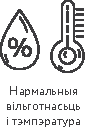
\includegraphics[scale=1.5]{willpower/ch11/12.pdf}
\end{figure}

\subsection*{Як кантраляваць вільготнасьць}

Каб вымераць вільготнасьць у~памяшканьні, скарыстайцеся адмысловым прыборам, які называецца гідрамэтар. Як правіла, датчык убудоўваецца ва ўвільгатняльнікі, у~вас можа быць некалькі датчыкаў у~розных памяшканьнях для паасобнага кантролю. Ёсьць спэцыяльныя асушальнікі паветра, ёсьць ультрагукавыя ўвільгатняльнікі паветра, і можна лёгка падтрымліваць неабходны ўзровень вільготнасьці ў~доме. Дасьледаваньні паказваюць, што павелічэньне вільготнасьці да 40\,\% здымае сымптомы раздражненьня. Оптымум вільготнасьці 40--60\,\%, занадта высокая вільготнасьць непажаданая, бо можа выклікаць шэраг іншых праблемаў. Выкарыстаньне буфэрных дыхальных матэрыялаў, накшталт мінімальна апрацаванага дрэва ці гіпсавых канструкцый, дазваляе ім убіраць лішак вільгаці з~паветра і затым, пры высыханьні, аддаваць.

\subsection*{Пытаньні і заданьні}

1. Які ўзровень вільготнасьці ў~вас у~памяшканьні?

2. Як вы пачуваецеся пры высокай і нізкай вільготнасьці?

3. Піце дастаткова вады, гэта дапамагае целу падтрымліваць водны балянс і цеплаабмен.


\section{Пазьбягайце кантакту з~таксінамі}

Як мудра заўважыў нямецкі паэт Готхальд Эфраім Лесінг, «яд, які ня дзейнічае адразу, не становіцца менш небясьпечным». У пачатку разьдзелу мы казалі пра таксічны фарбавальнік XIX стагоддзі на аснове мыш'яку, цяпер жа нас атачае нашмат большая колькасьць злучэньняў, часта не да канца вывучаных. Многія эфэкты злучэньняў праяўляюцца не адразу, а~па меры назапашваньня, і іх таксічнасьць сумуецца.

\emph{Хатні пыл, напрыклад, можа ўтрымліваць у~сабе полібрамаваныя дыфэнілэтэры, якія зьяўляюцца дадаткамі супраць гарэньня. З асьцярожнасьцю пастаўцеся да старых плястыкаў і дэкаратыўных вырабаў, яны могуць утрымліваць ужо забароненыя сёньня кампанэнты. Аддавайце перавагу прыродным матэрыялам у~дызайне і адзеньні, гэта найлепшае рашэньне.}

Асаблівую пагрозу для здароўя ўяўляюць так званыя \textbf{эндакрынныя дызраптары}~--- рэчывы, якія маюць гармонападобныя эфэкты. Ёсьць дызраптары, якія ўплываюць на палавыя залозы, парушаюць працу шчытавіцы, правакуюць назапашваньне тлушчу і павялічваюць рызыку цукровага дыябэту. Бісфэнол А ўваходзіць у~склад шматлікіх плястмасаў і зьяўляецца самым вывучаным з~дызраптараў. Ён вядзе да павелічэньня рызыкі дыябэту, раку падкарэньніцы і малочных залозаў, зьніжае фэртыльнасьць і спэрматагенэз. Дыяксіны могуць прыводзіць да бясплодзьдзя, парушэньня імунітэту. Поліхляраваныя біфэнілы (ПХБ) павялічваюць рызыку ўзьнікненьня раку скуры. Фталяты могуць трапляць зь мяккіх цацак, пакрыцьцяў падлогі ды іншых крыніцаў, выклікаючы парушэньне функцыянаваньня мужчынскай палавой сыстэмы.

\emph{Самымі небясьпечнымі лічаць дыбутылфталят (плястыфікатар для полівінілхлярыду), піраклястрабін (фунгіцыд), TBPDP (сродак для зьніжэньня гаручасьці з~дываноў). Мы можам атрымліваць гэтыя рэчывы рознымі шляхамі: зь ежай, вадой, паветрам, касмэтычнымі сродкамі і да т.~п. Устойлівыя арганічныя забруджвальнікі дыяксіны і поліхляраваныя біфэнілы (гексахлёрбіфэніл, гептахлёрадыбэнзвдыяксін, аксіхлярдан і іншыя) могуць назапашвацца ў~тлушчы: як у~харчовых ланцугах і ў~тлушчавай тканцы чалавека. Назапашваючыся, яны ўзмацняюць запаленьне, узьдзейнічаюць таксічна. Таксама многія з~гэтых злучэньняў стымулююць назапашваньне тлушчу, таму атрымалі назву абэсагены («стымулятары атлусьценьне»). Абэсагены спрыяюць павелічэньню колькасьці тлушчавых клетак, павышаючы схільнасьць да атлусьценьня. Калі чалавек худнее, то пры памяншэньні запасаў тлушчавай тканкі гэтыя злучэньні трапляюць у~крывацёк і могуць таксічна ўзьдзейнічаць.}

\textbf{Аднаразовае і небясьпечнае.} Звычайныя папяровыя кубачкі для гарбаты і кавы, папяровыя талеркі~--- гэта крыніца мікраплястыка, бо ўнутры яны пакрытыя плястыкам. Пры кантакце з~гарачай вадой адзін кубак выдзяляе ў~ваду 25 тысячаў часьціц мікраплястыку, якія зьмяшчаюць акрамя ўсяго яшчэ й іёны цяжкіх мэталаў. Гэтаксама паводзяцца і пакуначкі для гарбаты. Купляйце гарбату на вагу, запарвайце ў~імбрычку ці ў~мэталічных шматразовых «пакеціках».

Частай крыніцай таксінаў зьяўляецца і тэрмапапера, на якой друкуюць чэкі. Дастаткова 5 сэкундаў, каб 1 мг бісфэналу А пратачыўся ў~вашую скуру. А калі ў~вас рукі вільготныя ці змазаныя крэмам, то хуткасьць усмоктваньня яшчэ вышэйшая. Не бярыце чэкі ці бярыце іх пальчаткамі або праз складзеную паперу. Калі ў~вас у~офісе ці пакоі варта лязэрная друкарка, то гэта таксама небясьпечна для здароўя. У склад тонэра ўваходзяць цяжкія мэталы і небясьпечныя арганічныя злучэньні. Таму трымайце прынтэр у~асобным пакоі з~добрай вэнтыляцыяй, праветрывайце пасьля друку. Не ўжывайце пятнавыводнікі для канапаў і дываноў, плястыкі з~моцным пахам, асьвяжальнікі паветра і кандыцыянэры для бялізны, а~тасама любыя іншыя сынтэтычныя прадукты, якія не зьяўляюцца жыцьцёва неабходнымі.

\textbf{Забруджваньне прадуктаў}~--- гэта сур'ёзная крыніца таксінаў, але вымераць іх забруджанасьць складана: калі вырошчваць гародніну каля дарог, то ўтрыманьне цяжкіх мэталаў будзе падвышанае, а~вось за 100 мэтраў ад іх~--- ужо ў~норме. Прадукты могуць быць забруджаныя, калі іх паліваць вадой з~вадаёмаў, куды скідаюцца таксічныя адкіды. Пэстыцыды выкарыстоўваюцца вельмі часта, але звонку гэта выявіць немагчыма, таму мае сэнс давяраць правераным пастаўнікам і вытворцам, якія шануюць сваё імя.

Больш натуральных матэрыялаў. Аддавайце перавагу натуральным матэрыялам у~дызайне дома: тканінам, скуры, каменю, дрэву, мэталу~--- яны бясьпечныя, даўгавечныя і прыгожыя. Пачніце з~таго, што лёгка замяніць,~--- напрыклад, са штораў. Вельмі важна стварыць хатняе асяродзьдзе без выкарыстаньня патэнцыйна таксічных матэрыялаў. Напрыклад, драўняна-стружкавыя і драўняна-валанкністыя пліты, якія выкарыстоўваюцца для вырабу мэблі, могуць быць крыніцай фармальдэгіду і фэнолаў, прычым выдзяляюцца яны працяглы час. Танныя лямінаты, лінолеўм, плястык могуць уплываць гэтак жа. 

\emph{У сваёй кватэры мы зрабілі падлогу з~дошак~--- гэта зручна і бясьпечна.}

\begin{figure}[htb!]
  \centering
  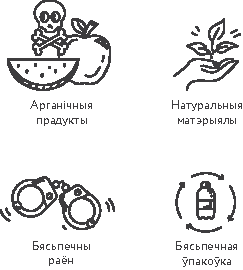
\includegraphics[scale=1.5]{willpower/ch11/13.pdf}
\end{figure}

Пакуйце і захоўвайце прадукты хаты ў~шкляным, а~ня плястыкавым посудзе. Плястыкавая тара, асабліва пры награваньні ці паўторным выкарыстаньні, узмацняе выдзяленьне небясьпечных злучэньняў. Не бярыце рукамі і не захоўвайце касавыя чэкі, не друкуйце шмат на прынтэры ў~жылых памяшканьнях або праветрывайце іх пасьля друку. Выкарыстоўвайце арганічныя туалетныя прыналежнасьці без фталатаў і іншых небясьпечных злучэньняў.

\emph{Сярод цяжкіх мэталаў прыярытэтнымі забруджвальнікамі лічацца волава, кадмій, цынк~--- галоўным чынам таму, што тэхнагеннае іх назапашваньне ў~навакольным асяродзідзі ідзе высокімі тэмпамі. Многія баяцца ртуці, дакладней мэтылртуці, якая зьяўляецца небясьпечным таксінам. Яе шмат у~некаторых морапрадуктах, у~глебах прамысловых рэгіёнаў, некаторых фарбавальніках. Таму лепш купляць рыбу невялікіх памераў (не пасьпяваюць назапасіць шмат ртуці) і з~тых відаў, якія не знаходзяцца на вяршыні харчовага ланцуга. А вось марскі акунь, рыба-меч, каралеўскі тунец, акула могуць утрымліваць багата ртуці.}

\subsection*{Пытаньні і заданьні}

1. Якія сынтэтычныя вырабы ў~вас дома можна замяніць на натуральныя? Што са старых рэчаў можна выкінуць ці вывезці з~дому?

2. Аддайце перавагу прадуктам харчаваньня з~больш бясьпечных крыніц.

3. Якіх паверхняў вы кранаецеся голай скурай? Ідэальна насіць адзеньне і сядзець на паверхнях і тканінах з~натуральных матэрыялаў.


\section{Дрэннае асьвятленьне}

Пагроза для здароўя ў~тым, што спэктар і інтэнсіўнасьць штучнага сьвятла моцна адрозьніваюцца ад сонечнага. Адыліж наша вока~--- гэта практычна частка мозгу, вынесеная на пэрыфэрыю! Штучнае сьвятло мае нізкую колераперадачу, часта яго крыніцы пульсуюць, ён мае спэктар выпраменьваньня без ультрафіялету, часта зь лішкам хваляў сіняга спэктру і з~дэфіцытам чырвонага, характарызуецца слабой інтэнсіўнасьцю ў~параўнаньні з~сонцам. Многія лямпы маюць ірваны спэктар у~адрозьненьне ад цэльнага сонечнага. Усё гэта стварае шматлікія пагрозы для здароўя: парушэньне выпрацоўкі мэлятаніну, пагаршэньне выпрацоўкі дафаміну і сератаніну, павышэньне нагрузкі на зрокавы апарат, збой цыркадных рытмаў. Усё гэта павялічвае рызыку шматлікіх захворваньняў, ад дыябэту і дэпрэсіі да хваробы Паркінсана. Калі ўжо мы змушаныя знаходзіцца пры штучным асьвятленьні, важна яго зрабіць як мага бясьпечнейшым для здароўя. Давайце разьбяромся, як правільна абраць найболей здаровую лямпу для дому: сьветлавая плынь, спэктар, колеравая тэмпэратура, колераперадача, пульсацыя.

\textbf{Адрэгулюйце колькасьць сьвятла.} Частая праблема памяшканьняў~--- малая колькасьць сьвятла, цьмянае сьвятло можа пагаршаць настрой і зьніжаць энэргічнасьць. Сьветлавая плынь~--- гэта колькасьць сьвятла, яна вымяраецца ў~люменах, як правіла, паказана на самой лямпе. Яркае сьвятло добрае раніцай і днём, яно бадзёрыць і падтрымлівае тонус. Старайцеся падбіраць сьвятло ня менш за 200--250 люмен на квадратны мэтар, гэта значыць, што тры лямпачкі на пакой будзе занадта мала. У зале ў~мяне 9 лямпаў па 500 люксаў, і стае іх толькі на цэнтар пакоя. На вуліцы нават у~пахмурнае надвор'е~--- 1000 люмен, а~ў сонечны дзень~--- 10.000 лм. Вымераць сьветлавую плынь можна люксомэтрам, прыблізна ацаніць камерай тэлефона, напрыклад з~праграмай Lux light meter. Нашыя вочы адаптуюцца да розных узроўняў асьветленасьці, таму візуальна параўноўваць даволі складана.

\textbf{Спэктар сьвятла лямпы.} Спэктар бывае бесьперапынным, як у~сонца ці лямпы напальваньня, ці рваным, калі ў~ім некалькі палосаў. Таксама вылучаюць спэктры зь перавагай рознага сьвятла. Большасьць сьвятлодыёдных лямпаў маюць скажоны спэктар зь сінім пікам. Гэта можа нэгатыўна паўплываць як на выпрацоўку мэлятаніну ўвечары, так і парушыць рэгуляцыю працы вока, бо да сіняга сьвятла асабліва адчувальныя гангліёзныя клеткі. У нашай сятчатцы ёсьць адмысловыя гангліянарныя мэлянапсінавыя клеткі, ад іх па рэтынагіпаталамічным шляху ў~гіпаталямус ідзе сыгнал, які кіруе цыркаднымі рытмамі і адказвае рэакцыю звужэньня зрэнак на сьвятло. Гэтыя клеткі ўзбуджаюцца сінім сьвятлом у~480 нм, таму «пік» у~звычайных сьвятлодыёдных лямпах можа зьбіваць наш унутраны гадзіньнік. Найлепшыя сьвятлодыёдныя лямпы сёньня~--- на аснове тэхналёгіі sunlike, іх спэктар бліжэйшы да сонечнага, бяз сіняга піку і правалу чырвонага. Увечары ж карысьнейшыя лямпы напальваньня, яны ня маюць піку сіняга сьвятла і асабліва не замінаюць выпрацоўцы мэлятаніну.

\textbf{Колеравая тэмпэратура}~--- гэта ўспрымальны колер лямпы. 4000К~--- гэта ``нэўтральны белы'', мякчэйшы жоўты 2700--2800К, а~высокая сьветлавая тэмпэратура вышэй 5500К можа раздражняць і стамляць.

\textbf{Колераперадача.} Ці часта было так, што вы купляеце прыгожую садавіну на рынку, а~на кухні яна выглядае нясмачна? А ваш твар зямлістым? Не сьпяшайцеся вінаваціць сябе ці прадаўцоў, праблема можа быць у~вашым хатнім асьвятленьні. Колераперадача~--- гэта параўнаньне, як выглядаюць адценьні ў~параўнаньні з~сонечным сьвятлом, наколькі раўнамерны ўзровень розных каляровых кампанэнтаў у~сьвятле. У сонца паказьнік колераперадачы 100 (CRI, Ra), а~ў лямпы чым больш CRI, тым лепш. Гэтае значэньне павінна быць пазначанае на ўпакоўцы. Калі CRI ніжэй ці роўны 80, то гэта шкодна, бо адценьні зьліваюцца, а~паніжэньне кантраснасьці ўспрымаецца нашым мозгам як страта рэзкасьці, і гэта змушае нас напружваць цягліцы вачэй, што вядзе да аўтаматычнай напругі вачэй, стамляльнасьці. У мяне стаяць лямпы з~CRI 95 і вышэй, і розьніца са звычайнымі прыкметная.

\textbf{Пульсацыя лямпы.} Чым вышэй пульсацыя лямпы, тым мацнейшая стомленасьць вачэй і горшае агульнае самаадчуваньне. Праверце лямпу праз камэру смартфона, навядзіце камэру на лямпу. Калі вы бачыце палосы ці пульсацыю сьвятла, то такая лямпа можа нэгатыўна ўплываць на вас. Часам на лямпе пазначана ``без пульсацыі''.

\textbf{Святлодызайн.} Найлепшае сьвятло~--- дзённае. Таму аптымальна часьцей быць на вуліцы, абыходзіцца мінімумам штораў, цюляў, фіранак, аб'ёмных расьлінаў, якія засланяюць плынь сьвятла. Чым большыя вокны~--- тым лепш. Можна працаваць ці выходзіць на гаўбец, дах, тэрасу. Часам выкарыстоўваюць сьвятлаводы, каб накіраваць сонечнае сьвятло ўглыб будынкаў. Для лепшага сьвятла ў~памяшканьні часта выкарыстоўваюць камбінацыю розных крыніцаў сьвятла, удома таксама мае сэнс выкарыстоўваць як дзённае, так і вечаровае (ніжняе, зь лямпамі напальваньня) сьвятло.

Можна яшчэ выкарыстоўваць для лепшай асьветленасьці і дызайн. Так, у~мяне ў~кватэры~--- белыя сьцены і столь, белая падлога з~глянцавай фарбай. Белыя і гладкія паверхні маюць большы каэфіцыент адлюстраваньня сьвятла, чым цёмныя і шурпатыя. І не выпадкова скандынаўскі дызайн узьнік для таго, каб кампэнсаваць недахоп сьвятла.

\subsection*{Пытаньні і заданьні}

1. Вымерайце з~дапамогай праграмы асьветленасьць у~пакоі, на вашым працоўным стале. Ці стае вам сьвятла? Калі не~--- павялічце яркасьць у~сябе дома.

2. Параўнайце сваё колеравае ўспрыманьне аднаго і таго ж прадмета ў~заштораным пакоі са сьвятлом і выносячы яго на гаўбец пад сонца.

3. Вымыйце вокны і пазбаўцеся ўсяго, што перашкаджае сонечным прамяням. Па магчымасьці перанясіце ваша працоўнае месца бліжэй да акна. Ці паўплывала гэта на вашую прадуктыўнасьць?

\clearpage
\thispagestyle{empty}
\begin{figure}[htb!]
  \vspace*{-0.25in}
  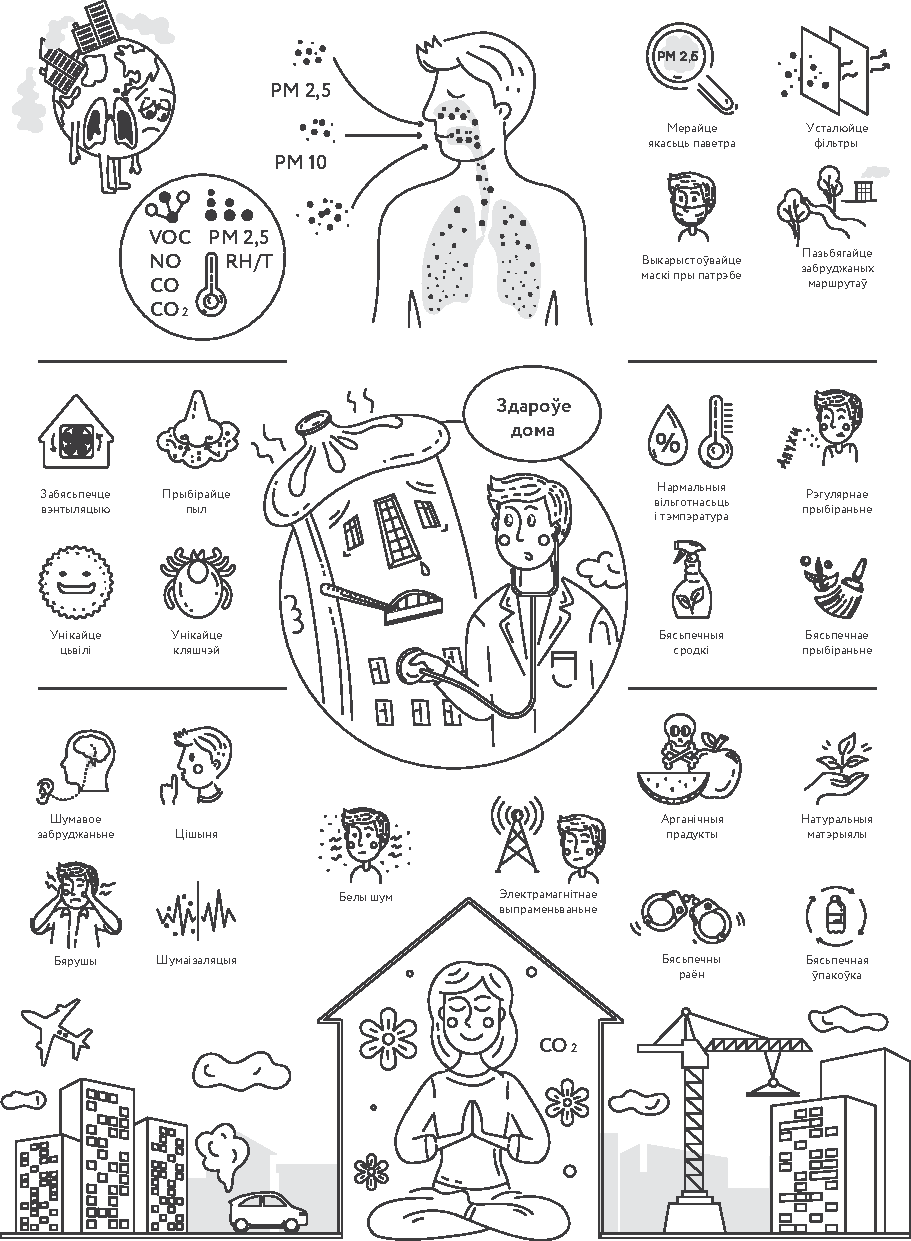
\includegraphics[width=\textwidth]{willpower/ch11/full.pdf}  
\end{figure}
